\documentclass[a4paper,12pt,hyphens,oneside]{report}
\usepackage{xcolor}
\usepackage{color}
\usepackage[unicode,linktocpage]{hyperref}
\usepackage{tocbibind}
\usepackage[toc,titletoc]{appendix}
\hypersetup{backref,colorlinks=true, urlcolor=green, linkcolor=black, unicode=true}
\hypersetup
{
    pdfauthor={Cao Văn Phúc},
    pdftitle={Tìm hiểu giải thuật tìm kiếm cục bộ dựa trên ràng buộc và cài đặt
bài toán đóng thùng 2D sử dụng thư viện JOpenCBLS}
}

\usepackage{ifluatex}

\ifluatex % LuaTeX
  \usepackage{luatextra}
  \usepackage{fontspec}
  \defaultfontfeatures{Ligatures=TeX}
  % load your system fonts; e.g.:
 \setmainfont{Times New Roman}
  %\setmainfont{LinLibertineO}
  %\setsansfont{LinBiolinumO}
  %\setmonofont{Inconsolata}
  \usepackage{polyglossia}
  \setdefaultlanguage{vietnamese}

  \newfontfamily\arial{Arial}
\else % pdfTeX
  \usepackage[utf8]{inputenc}
  \usepackage[utf8]{vietnam}
  %\usepackage[T1]{fontenc}
  % load some Type 1 font; e.g.:
  \usepackage[fulloldstylenums,largesmallcaps]{kpfonts}
\fi

\PassOptionsToPackage{hyphens}{url}\usepackage{hyperref}
\usepackage[ruled,vlined]{algorithm2e}
\usepackage{algorithmic}
\usepackage{latexsym, amsfonts, amssymb, amsmath, amsthm}
%\usepackage{enumitem}
\usepackage{cases}
\usepackage{empheq}
\usepackage[left=3.5cm,right=2.0cm,top=2.0cm,bottom=2.0cm,includefoot,includehead,heightrounded]{geometry}
\usepackage{fancybox}
\usepackage{titlesec}
\usepackage{listings}
\usepackage{frame}
\usepackage{framed}
\usepackage{graphicx}
\usepackage{caption}
\usepackage{subcaption}
\usepackage{verbatim}
\usepackage{fancyhdr}
\usepackage{multirow}
\usepackage{float}
\usepackage{tabularx}
\usepackage{threeparttable}
\usepackage[xindy,toc]{glossaries}
\usepackage{tabu}
\usepackage{linegoal}
%\usepackage{natbib}
\usepackage{array}
\usepackage{indentfirst}
\usepackage{booktabs}
\usepackage{siunitx}
\usepackage{listings}

%%%%%%%%%%%%%%% Listings %%%%%%%%%%%%%%%%%%%%%%%%%%%%%%%%%%
%\lstset{inputencoding=utf8,extendedchars=true,language=java}

\definecolor{dkgreen}{rgb}{0,0.6,0}
\definecolor{gray}{rgb}{0.5,0.5,0.5}
\definecolor{mauve}{rgb}{0.58,0,0.82}

\lstdefinelanguage{json}{
    basicstyle=\normalfont\ttfamily,
    numbers=left,
    numberstyle=\scriptsize,
    stepnumber=1,
    numbersep=8pt,
    showstringspaces=false,
    breaklines=true,
    frame=lines,
    backgroundcolor=\color{background},
    literate=
     *{0}{{{\color{numb}0}}}{1}
      {1}{{{\color{numb}1}}}{1}
      {2}{{{\color{numb}2}}}{1}
      {3}{{{\color{numb}3}}}{1}
      {4}{{{\color{numb}4}}}{1}
      {5}{{{\color{numb}5}}}{1}
      {6}{{{\color{numb}6}}}{1}
      {7}{{{\color{numb}7}}}{1}
      {8}{{{\color{numb}8}}}{1}
      {9}{{{\color{numb}9}}}{1}
      {:}{{{\color{punct}{:}}}}{1}
      {,}{{{\color{punct}{,}}}}{1}
      {\{}{{{\color{delim}{\{}}}}{1}
      {\}}{{{\color{delim}{\}}}}}{1}
      {[}{{{\color{delim}{[}}}}{1}
      {]}{{{\color{delim}{]}}}}{1},
}

\lstset{frame=tb,
  language=Java,
  aboveskip=3mm,
  belowskip=3mm,
  showstringspaces=false,
  columns=flexible,
  basicstyle={\small\ttfamily},
  numbers=none,
  numberstyle=\tiny\color{gray},
  keywordstyle=\color{blue},
  commentstyle=\color{dkgreen},
  stringstyle=\color{mauve},
  breaklines=true,
  breakatwhitespace=true,
  tabsize=4
}
%%%%%%%%%%%%%%% BibTex %%%%%%%%%%%%%%%%%%%%%%%%%%%%%%%%%%%%
%\makeatletter
%\newrobustcmd*{\mkbibitalic}{\textit}
%\protected\long\def\blx@imc@mkbibemph#1{%
%  \textit{#1}\blx@imc@setpunctfont\textit}
%\makeatother
%
%\let\mkbibemph\mkbibitalic

%%%%%%%%%%%%% Glossaries %%%%%%%%%%%%%%%%%%%%%%%%%%%%%%%%%
\makeglossaries

%\usepackage{setspace}
%\onehalfspace

%%%%%%%%%% THEOREM %%%%%%%%%%%%%%%%%%%%%%%%%%%%%%%%%%%%%%%%
\newtheorem{theorem}{Theorem}[section]
\newtheorem{lemma}[theorem]{Lemma}
\newtheorem{proposition}[theorem]{Proposition}
\newtheorem{corollary}[theorem]{Corollary}

%\newenvironment{proof}[1][Proof]{\begin{trivlist}
%\item[\hskip \labelsep {\bfseries #1}]}{\end{trivlist}}
\newenvironment{definition}[1][Định nghĩa]{\begin{trivlist}
\item[\hskip \labelsep {\bfseries #1}]}{\end{trivlist}}
\newenvironment{example}[1][Example]{\begin{trivlist}
\item[\hskip \labelsep {\bfseries #1}]}{\end{trivlist}}
\newenvironment{remark}[1][Remark]{\begin{trivlist}
\item[\hskip \labelsep {\bfseries #1}]}{\end{trivlist}}

%\newcommand{\qed}{\nobreak \ifvmode \relax \else
%      \ifdim\lastskip<1.5em \hskip-\lastskip
%      \hskip1.5em plus0em minus0.5em \fi \nobreak
%      \vrule height0.75em width0.5em depth0.25em\fi}

%%%%%%%%%% TIKZ settings %%%%%%%%%%%%%%%%%%%%%%%%%%%%
\usepackage{tikz}
%\usepackage{unicode-math}
\usepackage{pgfplots}
\usepackage{pgfplotstable}
\usepackage{calc}

\pgfplotsset{compat=1.12}

\usetikzlibrary{arrows,shapes,calc}
\usetikzlibrary{patterns}

\tikzstyle{vertex}=[circle,fill=black!25,minimum size=10pt,inner sep=0pt]
\tikzstyle{selected vertex} = [vertex, fill=red!24]
\tikzstyle{next vertex} = [vertex, fill=yellow!24]
\tikzstyle{edge} = [draw,thick,-]
\tikzstyle{weight} = [font=\small]
\tikzstyle{selected edge} = [draw,line width=5pt,dotted,red!50]
\tikzstyle{new edge} = [draw,line width=3pt,-,green!50]
\tikzstyle{ignored edge} = [draw,line width=5pt,-,black!20]

\tikzstyle{redcell}=[rectangle,pattern=north west lines,pattern color=red,fill opacity=0.1]
\tikzstyle{blackcell}=[rectangle,pattern=dots,pattern color=black,fill opacity=0.3]
\tikzstyle{celllabel}=[midway,opacity=1,font=\normalsize]
\tikzstyle{edgelabel}=[midway,opacity=1,fill=white,font=\normalsize]

% Declare layers
\pgfdeclarelayer{background}
\pgfsetlayers{background,main}

% caption source
\newcommand*{\captionsource}[2]{%
  \caption[{#1}]{%
    #1%
    \\\hspace{\linewidth}%
    \textbf{Nguồn:} #2%
  }%
}

%%%%%%%%%%%%%%%%%%%%%%%%%%%%%%%%%% vietnamese names
%\def\captionsvietnamese{%
%\def\listtablename{Danh sách bảng}%
%}%
\addto\captionsvietnamese{%
  \renewcommand{\listtablename}{Danh sách bảng}%
  \renewcommand{\listfigurename}{Danh sách hình ảnh}%
  \renewcommand{\contentsname}{Mục lục}%
  \renewcommand{\tablename}{Bảng}%
  \renewcommand{\glossaryname}{Danh sách thuật ngữ và từ viết tắt}%
  \renewcommand{\appendixtocname}{Phụ lục}%
  \renewcommand{\appendixpagename}{Phụ lục}%
}%

%%%%%%%%%%%%%%%%%%%%%%%%%%%%%%%%%%%%%%%%%%%%%%%%%%%%%

% section depth
\setcounter{secnumdepth}{5}
\setcounter{tocdepth}{5}

\setlength{\headheight}{27pt}

\newcommand{\credit}[1]{
\\
\hspace*{15pt}
\hbox{\scriptsize Credit:\thinspace{\small\itshape \scriptsize #1}}}


    \makeatletter
    % avoid the redefinition of `\thepart`
    \patchcmd{\captionsfrench}{\def\thepart{}}{}{}{}
    % patch \@part not to print the part number
    \patchcmd{\@part}{\nobreakspace\thepart}{}{}{}
    \makeatother

% line spacing
\linespread{1.2}

% footnote
\makeatletter
\newcommand \Dotfill {\leavevmode \cleaders \hb@xt@ .2em{\hss .\hss }\hfill \kern \z@}
%\renewcommand{\chaptermark}[1]{%
%    \markboth{\@chapapp\ \thechapter.\ #1}{}
%}%


\makeatother
\fancypagestyle{plain}{
    \fancyfoot{} % clear all footer fields
    \renewcommand{\headrulewidth}{0.1pt}
    \renewcommand{\footrule}{\vbox to 0pt{\hbox to\headwidth{\Dotfill}\vss}}
    \renewcommand{\headrule}{\vbox to 0pt{\hbox to\headwidth{\Dotfill}\vss}}
    \renewcommand{\footrulewidth}{0.1pt}
    \fancyfoot[R]{\thepage}           % page number in "outer" position of footer line
    \fancyfoot[L]{\textit{\footnotesize Sinh viên thực hiện: Cao Văn Phúc - 20102715 Khóa K55 Lớp CNTT4}} % other info in "inner" position of footer line

    \rhead{\leftmark}
    \lhead{\rightmark}
}%
\fancypagestyle{title}
{
    \fancyhf{}
    \renewcommand\headrulewidth{0pt}
    \renewcommand\footrulewidth{0.1pt}
    \renewcommand{\footrule}{\vbox to 0pt{\hbox to\headwidth{\Dotfill}\vss}}
    \fancyfoot[L]{\textit{\footnotesize Sinh viên thực hiện: Cao Văn Phúc - 20102715 Khóa K55 Lớp CNTT4}} % other info in "inner" position of footer line
}

%%%%%%%% TABLES %%%%%%%%%%%%%%%%%%%%%%%%%%%%%%%%
\newcolumntype{P}[1]{>{\centering\arraybackslash}p{#1}}

%%%%%%%% Grouping figure/table %%%%%%%%%%%%%%%%%
\usepackage{etoolbox}
\makeatletter
\def\thischaptertitle{}
\apptocmd{\@chapter}{\gdef\thischaptertitle{#1}}{}{}

\newcommand{\DeclareDividedList}[1]%
  {\newcounter{#1@chapter}\setcounter{#1@chapter}{0}}

\pretocmd{\addcontentsline}%
  {\ifltxcounter{#1@chapter}%
   {%
     \ifnumgreater{\thechapter}{\value{#1@chapter}}{%
       \setcounter{#1@chapter}{\thechapter}%
       \addtocontents{#1}{\protect\contentsline{chapter}%
         {\protect\numberline {\thechapter} {\thischaptertitle}}{}{} }
     }{}%
   }{}%
  }{}{}
\makeatother
\DeclareDividedList{lof}
%\DeclareDividedList{lot}

%%%%%%%%%%%%%%%%%%%%%%%%%%%%%%%%%%%%%%%%%%%%%%%%%%%%%%%%%%%%%%%%%%%%%%%%%%%%%%%%%%%%%%%%%%%
\begin{document}

    \title{\color{red} Giải thuật tìm kiếm cục bộ dựa trên ràng buộc giải bài toán đóng thùng 2D}
    \author{\color{blue}Cao Văn Phúc}
    \date{\color{green}\today}
	\nocite{*}	
	
    \begin{titlepage}
        \thispagestyle{empty}
        \newgeometry{left=3.7cm,bottom=2.1cm,right=2.2cm,top=2cm,includefoot}
        \begin{tikzpicture}[remember picture, overlay]
          \draw[line width = 0.5pt] ($(current page.north west) + (3.5cm,-2cm)$) rectangle ($(current page.south east) + (-2cm,2cm)$);
        \end{tikzpicture}

        \begin{center}
            {\fontsize{16}{1.2}\selectfont TRƯỜNG ĐẠI HỌC BÁCH KHOA HÀ NỘI\\
            VIỆN CÔNG NGHỆ THÔNG TIN VÀ TRUYỀN THÔNG}
        \textbf{--------------------  *  ---------------------}\\[3.8cm]
        %
\includegraphics[width=3cm, height=4.2cm]{figures/logo}\\[1cm]
        {\fontsize{32pt}{1}\selectfont ĐỒ ÁN}\\
        {\fontsize{38pt}{1}\selectfont \textbf{TỐT NGHIỆP ĐẠI HỌC}}\\[0.8cm]
        {\fontsize{20pt}{1}\selectfont NGÀNH CÔNG NGHỆ THÔNG TIN}\\[3.0cm]
        {\fontsize{22pt}{1}\selectfont Giải thuật tìm kiếm cục bộ dựa trên ràng buộc\\
         giải bài toán đóng thùng 2D
        }\\[2.8cm]
        \end{center}

        {\fontsize{14pt}{1}\selectfont
            \hspace*{4.5cm} Sinh viên thực hiện: \hspace{4pt} \textbf{\parbox[t]{5cm}{
                     Cao Văn Phúc\\
                     Lớp CNTT4 - K55}
            }\\[12pt]
        }
        {\fontsize{14pt}{1}\selectfont
            \hspace*{4.5cm} Giảng viên hướng dẫn:  \hspace{4pt} \textbf{\parbox[t]{5cm}{
                    TS. Phạm Quang Dũng\\}
            }
        }

        \vspace{3.5cm}
        \begin{center}
        {\fontsize{16pt}{1}\selectfont HÀ NỘI \luaexec{tex.print(os.date("\%m - \%Y"))}}\\
        \end{center}
    \end{titlepage}

    \restoregeometry
    \newpage
    %\pagenumbering{Alph}

    \pagestyle{title}
    \addcontentsline{toc}{chapter}{PHIẾU GIAO NHIỆM VỤ ĐỒ ÁN TỐT NGHIỆP}
\newgeometry{left=3.5cm,bottom=2cm,right=2cm,top=2cm,includefoot}
{\fontsize{14}{1}\selectfont\centering\bfseries
    PHIẾU GIAO NHIỆM VỤ ĐỒ ÁN TỐT NGHIỆP
\par}%

\fontsize{12}{14.4}
\selectfont

{\noindent
\setlength{\parindent}{0pt}

1. Thông tin về sinh viên\\
Họ và tên: Cao Văn Phúc \hspace{4.6cm} Email: phuccaotp@gmail.com\\
Lớp: CNTT4 \hspace{7.6cm} Hệ đào tạo: Chính quy\\
Đồ án tốt nghiệp được thực hiện tại: Phòng 902 - B1\\
Thời gian làm ĐATN: Từ ngày 20/02/2015 đến 20/08/2015\\
\\
2. Mục đích nội dung của ĐATN\\
Tìm hiểu giải thuật tìm kiếm cục bộ dựa trên ràng buộc và cài đặt
bài toán đóng thùng 2D (Bin Packing 2D) sử dụng thư viện JOpenCBLS.\\
\\
3. Các nhiệm vụ cụ thể của ĐATN
\begin{itemize}
    \item Tìm hiểu giải thuật tìm kiếm cục bộ giải các bài toán có ràng buộc,
    \item Tìm hiểu thư viện JOpenCBLS,
    \item Phát triển giải thuật tìm kiếm cục bộ để giải bài toán đóng thùng 2D,
    \item Cài đặt ứng dụng tương tác với người dùng,
    \item Thử nghiệm và đánh giá thư viện JOpenCBLS trên bài toán BP2D.
\end{itemize}

4. Lời cam đoan của sinh viên:\\
Tôi - \textit{Cao Văn Phúc} - cam kết ĐATN là công trình nghiên cứu của bản
thân tôi dưới sự hướng dẫn của học \textit{TS. Phạm Quang Dũng}.
Các kết quả nêu trong ĐATN là trung thực, không phải là sao chép toàn văn của
bất kỳ công trình nào khác.

\begin{table}[H]
    \centering
    \begin{tabular}{P{0.45\textwidth} P{0.45\textwidth}}
        & \textit{Hà Nội, \luaexec{tex.print(os.date("ngày \%d tháng \%m năm \%Y"))}}\newline
            Tác giả ĐATN\newline
            \newline
            \newline
          \textit{Cao Văn Phúc}\\
    \end{tabular}
\end{table}


5. Xác nhận của giáo viên hướng dẫn về mức độ hoàn thành của ĐATN và cho phép
bảo vệ:\\
\textit{Sinh viên đã hoàn thành tốt các nhiệm vụ của ĐATN đại học. Tôi đề nghị
        cho sinh viên được bảo vệ tốt nghiệp.}

\begin{table}[H]
    \centering
    \begin{tabular}{P{0.45\textwidth} P{0.45\textwidth}}
        %& \textit{Hà Nội, \luaexec{tex.print(os.date("ngày \%d tháng \%m năm \%Y"))}}\newline
        & \textit{Hà Nội, \luaexec{tex.print(os.date("ngày 28 tháng \%m năm \%Y"))}}\newline
            Giáo viên hướng dẫn\newline
            \newline
            \newline
          \textit{TS. Phạm Quang Dũng}\\
    \end{tabular}
\end{table}

}% noindent
\restoregeometry

    %\newpage

    \fontsize{13}{15.6}
    \selectfont

    \renewcommand{\chaptermark}[1]{\markboth{#1}{}}
    \renewcommand{\sectionmark}[1]{\markright{#1}{}}
    \renewcommand{\chaptermark}[1]{\markboth{\chaptername\ \thechapter.\ #1}{}}

    \rhead{\leftmark}
    \lhead{\rightmark}

    \pagestyle{plain}
    %\pagenumbering{Alph}
    \newglossaryentry{GPU}
{
    name=GPU,
    description={Graphic Processing Unit - Đơn vị xử lý đồ họa}
}

\newglossaryentry{pipeline}
{
    name=pipeline,
    description={hay \texttt{graphic pipeline} - đường ống đồ họa: một dãy các bước kế tiếp nhau trong quá trình xử lý đồ họa}
}

\newglossaryentry{shader}
{
    name=shader,
    description={Chương trình được GPU sử dụng cho một số bước trong pipeline}
}

\newglossaryentry{GPGPU}
{
    name=GPGPU,
    description={General-purpose computing on Graphics Processing Units - Tính
    toán mục đích thông dụng trên GPU}
}

\newglossaryentry{CUDA}
{
    name=CUDA,
    description={Compute Unified Device Architecture - một môi trường dành cho lập trình
    GPGPU trên các GPU của NVIDIA}
}

\newglossaryentry{kernel}
{
    name=Kernel,
    description={Chương trình C/C++ được gọi từ CPU để chạy trên mỗi thread của GPU}
}

\newglossaryentry{thread}
{
    name=thread,
    description={Luồng, hay luồng thực thi. Là một dãy các câu lệnh được thực
    thi một cách tuần tự trên CPU hoặc GPU}
}

\newglossaryentry{SM}
{
    name=SM,
    description={Stream Multiprocessor - Bộ đa xử lý dòng}
}

\newglossaryentry{SMX}
{
    name=SMX,
    description={Giống SM, nhưng dành cho GPU kiến trúc Kepler}
}

\newglossaryentry{block}
{
    name=block,
    description={Cũng gọi là thread block. Là một nhóm các thread của CUDA được
    thực thi trên cùng một SM}
}

\newglossaryentry{compute capability}
{
    name=compute capability,
    description={Khả năng tính toán. Một con số chỉ phiên bản, chức năng của
    một SM}
}

\newglossaryentry{Core}
{
    name=Core,
    description={Nhân CUDA, đơn vị cơ bản trực tiếp tính các phép tính số học,
    logic, dấu phẩy động trên GPU}
}

\newglossaryentry{warp}
{
    name=warp,
    description={Nhóm 32 thread CUDA liên tiếp trong cùng một block. Được điều
    phối công việc cùng nhau.}
}

\newglossaryentry{SIMT}
{
    name=SIMT,
    description={Single Instruction, Multiple Thread}
}

\newglossaryentry{SIMD}
{
    name=SIMD,
    description={Single Instruction, Multiple Data}
}

\newglossaryentry{HDF}
{
    name=HDF,
    description={Hydrodynamic Flow - Dòng chảy thủy động lực học}
}

\newglossaryentry{MAC}
{
    name=MAC,
    description={Marker-and-Cell, một phương pháp giải bài toàn HDF}
}

\newglossaryentry{CFD}
{
    name=CFD,
    description={Computational Fluid Dynamic - Tính toán động lực học chất lưu}
}

\newglossaryentry{occupancy}
{
    name=occupancy,
    description={Mức độ chiếm giữ - tỉ lê giữa số thread thực tế và tối đa có
    thể chạy trên 1 SM}
}


    \chapter*{Tóm Tắt Nội Dung Đồ Án Tốt Nghiệp}
%\addcontentsline{toc}{chapter}{\numberline{}Mở đầu}
\addcontentsline{toc}{chapter}{Mở đầu}
\markboth{Mở đầu}{}
Bài toán tối ưu tổ hợp là bài toán rất phổ biến trong đời sống xã hội, đặc biệt trong các lĩnh vực như phân công, quản lý, lập kế hoạch. Mục tiêu của các bài toán này là tìm một lời giải thỏa mãn một tập các ràng buộc được đặt ra và đồng thời có thể tối ưu một số mục tiêu nào đó. Thông thường các bài toán này đều thuộc lớp các bài toán NP-Khó, các phương pháp giải bài toán tối ưu tổ hợp được chia làm hai hướng: hướng tiếp cận đúng và hướng tiếp cận gần đúng.

Trong các hướng tiếp cận thì hướng tiếp cận gần đúng sẽ là khả thi hơn khi khối lượng tính toán trong các bài toán tối ưu này vượt xa khả năng tính toán của các máy tính hiện tại (2015) nếu theo hướng tiếp cận đúng. Phương pháp tìm kiếm cục bộ dựa trên ràng buộc là một phương pháp theo hướng tiếp cận gần đúng có thể sử dụng trong các bài toán tối ưu này.

Lớp các bài toán đóng thùng (Bin Packing) \cite{hopper2000twodimensional, lodi1999heuristic, ortmann2010newimpro, prisinger2005thetwod} là các bài toán liên quan đến việc xếp các vật phẩm với kích thước cho trước vào một số các thùng (Bin) thỏa mãn các ràng buộc không chồng lấn về mặt không gian và thực hiện tối ưu một số mục tiêu nào đó.

Đồ án này nghiên cứu tìm kiếm lời giải cho bài toán đóng thùng 2D với phương pháp tìm kiếm cục bộ dựa trên ràng buộc \cite{rossi2006handbookOfCp, pascal2005cp} sử dụng bộ thư viện JOpenCBLS \cite{dungpq2015cbls}.

Nội dung đồ án bao gồm:

\textbf{Chương \ref{chap:combOpt}} Giới thiệu về bài toán tối ưu hóa tổ hợp trong khoa học máy tính, các phương pháp tiếp cận, ưu nhược điểm và các kết quả thực tiễn. Phương pháp tìm kiếm cục bộ dựa trên ràng buộc, các kết quả và công việc còn phải thực hiện và giới thiệu về thư viện JOpenCBLS.

\textbf{Chương \ref{chap:binPacking}} giới thiệu về bài toán Bin Packing 2D: mô tả, mô hình toán học, ứng dụng của trong thực tiễn.

\textbf{Chương \ref{chap:implement}} phân tích, cài đặt cách thức thực hiện tìm kiếm cục bộ trên bài toán đóng thùng và áp dụng thư viện JOpenCBLS vào để giải bài toán đóng thùng 2D.

\textbf{Chương \ref{chap:presentation}} minh họa chương trình đã được cài đặt với thư viện JOpenCBLS với giao diện tương tác người dùng sử dụng công nghệ J2EE, Javascript, Bootstrap. Mục này bao gồm các kết quả thống kê trên các bộ dữ liệu kiểm tra có sẵn, kết quả trên các bộ này cho thấy chương trình cho khả năng giải tốt các bài này.


    \tableofcontents

    %\pagenumbering{arabic}

    \glsaddall
    \setglossarystyle{list}
    \printglossaries

    \listoffigures
    \listoftables

    %\hypersetup{linkcolor=blue}


    \renewcommand{\thefootnote}{\arabic{footnote}}

    \chapter*{Danh mục từ viết tắt\markboth{Danh mục từ viết tắt}{}}%
\addcontentsline{toc}{chapter}{Danh mục từ viết tắt}%

\begin{description}
    \item[CBLS] Constraint Base Local Search: thuật toán tìm kiếm cục bộ dựa trên ràng buộc.
    \item[JOpenCBLS] Thư viện tìm kiếm cục bộ dựa trên ràng buộc được thiết kế và phát triển bởi TS. Phạm Quang Dũng và các thành viên \textsc{lab Thuật toán và tối ưu - ĐH Bách Khoa Hà Nội}
    \item[BP] Bin Packing
    \item[BP2D] Bin Packing 2D
    \item[MVP] Kiến trúc Model-View-Presenter
    \item[CP] Constraint Programming: Quy hoạch ràng buộc.
\end{description}

    %\chapter*{Tóm tắt nột dung}%
\addcontentsline{toc}{chapter}{\numberline{}Tóm tắt nội dung}%
Quản lý file là một chức năng của hầu hết các hệ điều hành hiện nay. Tuy nhiên
hiện nay có nhiều hệ thống file (filesystem) khác nhau, mỗi hệ thống file có
những cách đọc, ghi dữ liệu khác nhau. Có những hệ thống file dành cho các
thiết bị lưu trữ vật lý, nhưng cũng có những hệ thống file dành riêng cho việc
chia sẻ qua mạng hay là lưu trữ trên bộ nhớ RAM.

Phần đầu bài báo cáo này tìm hiệu về hệ thống file ảo (VFS) trên Linux, một thành phần
của nhân Linux đóng vai trò là giao diện thống nhất tất cả các hệ thống file,
làm cho việc quản lý file trên Linux trở nên đơn giản hơn.

Phần hai của bài báo cáo tìm hiểu về bộ nhớ flash và hệ thống file F2FS dành
cho bộ nhớ flash. Cũng như nhiều hệ thống file khác trên Linux, cài đặt của
F2FS cũng sử dụng giao diện cung cấp bởi VFS. Qua việc tìm hiểu F2FS, ta sẽ
thấy quản lý file không phải chỉ cần quan tâm đến mức phần mềm mà còn phải biết tận dụng
các ưu điểm và khắc phục các nhược điểm của thiết bị lưu trữ phần cứng.

    \chapter{Bài Toán Tối Ưu Tổ Hợp}
\label{chap:combOpt}
%======================================================================
\section{Tổ hợp và không gian tìm kiếm}
\label{sec:co_space}

%-----------------------------------------------------------------
\subsection{Khái niệm}

\subsubsection*{Bài Toán Tối ưu tổ hợp}
Bài toán tối ưu tổ hợp \cite{pascal2005cp} là một dạng của bài toán tối ưu, nó có dạng tổng quát như sau:
\begin{itemize}
	\item Cho hàm $f(X)$ xác định trên một tập hữu hạn các phần tử $D$, hàm $f(x)$ được gọi là hàm mục tiêu.
	\item Mỗi phần tử $X$ thuộc $D$ có dạng $X=(x_1,\dots,x_n)$ được gọi là một phương án.
	\item Cần tìm một phương án $X$ thuộc $D$ sao cho hàm $f(X)$ đạt cực tiểu, phương án $X$ như vậy được gọi là phương án tối ưu.
\end{itemize}

\subsubsection*{Bài toán thỏa mãn ràng buộc}

Bài toán thỏa mãn ràng buộc \cite{pascal2005cp} là bài toán tối ưu tổ hợp bổ sung thêm các điều kiện ràng buộc được xác định bởi bộ
\[
\{X, D, C, F\}
\]
với:
\begin{description}
	\item $X = \{X_1,\dotsc, X_n\}$ \quad là tập các biến.
	\item $D = \{D_1,\dotsc, D_n\}$ \quad là tập miền xác định tương ứng của các biến.
	\item $C = \{C_1,\dotsc, C_m\}$ \quad là tập các ràng buộc.
	\item $F = \{F_1,\dotsc, F_k\}$ \quad là tập các hàm mục tiêu cần tối ưu.
\end{description}

Tập $S = \{t_1,\dotsc, t_n\}$ với phần tử $t_i$ là giá trị tương ứng của mỗi biến $X_i$ và $S$ thỏa mãn tất cả các ràng buộc định nghĩa trong $C$ thì $S$ được gọi là tập lời giải của bài toán thỏa mãn ràng buộc trên bộ $\{X, D, C\}$.

Trong nhiều bài toán chúng ta còn cần phải tối ưu thêm các mục tiêu:
\begin{equation}
F_i = f(X_1,\dotsc, X_n) \quad 1 \leq i \leq k.
\end{equation}
Lời giải $S^*$ trong tập các lời giải $S$ của bài toán thỏa mãn ràng buộc trên đồng thời cho giá trị cực tiểu của các hàm mục tiêu $F_i$ thì $S^*$ được gọi là lời giải tối ưu của bài toán.

\subsubsection*{Không gian tìm kiếm lời giải}
Tất cả các bài toán tối ưu tổ hợp đều có độ phức tạp tính toán hàm mũ, chúng thuộc lớp các bài toán \textsf{NP-khó} và chưa có các thuật toán hiệu quả để tìm kiếm lời giải.

%------------------------------------------------------------------
\subsection{Ví dụ}

\subsubsection*{N-QUEEN}

\begin{figure}
	\centering
	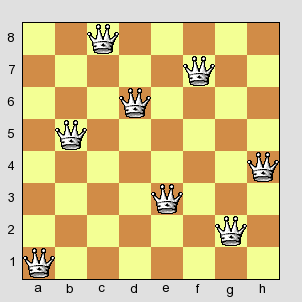
\includegraphics[scale=1]{figures/10-queens-sol.png}
	\caption{Lời giải của bài toán 8 con hậu \cite{PaulButler2009queens}.\label{fig:queens}}
\end{figure}

Bài toán sắp xếp $N ( N > 4)$ quân hậu yêu cầu sắp xếp $N$ quân hậu trên bàn cờ vua sao cho không có quân hậu nào có thể \textsc{ăn} được các quân hậu còn lại theo quy tắc cờ vua. Hay có thể phát biểu rằng không có hai con hậu nào cùng nằm tren một hàng, một cột hoặc một đường chéo.

Mô hình toán học:
\begin{list}{•}{}
	\item $X = \{x_i | 1 \le i \le N \}$ \quad với $x_i$ là chỉ số cột của con hậu hàng thứ $i$.
	\item $D = \{d_i | 1 \le i \le N \ | d_i \in \{1,2,\dots,N\}\}$ \quad là các miền giá trị của $x_i$.
	\item Tập các ràng buộc $C$:
	\[ C =
  		\begin{cases}
    		x_i \neq x_j, 1 \leq i < j \leq N       	 & \quad \text{Không có hai con hậu nào trên cùng một cột}\\
    		x_i - i \neq x_j - j, 1 \leq i < j \leq N  & \quad \text{Ràng buộc đường chéo thuận}\\		
    		x_i + i \neq x_j + j, 1 \leq i < j \leq N  & \quad \text{Ràng buộc đường chéo ngược}\\
  		\end{cases}
	\]
\end{list}

Hình \ref{fig:queens} là một phương án thỏa mãn ràng buộc của bài toán 10 con hậu:
\subsubsection*{Graph-Coloring}

\begin{figure}
	\centering
	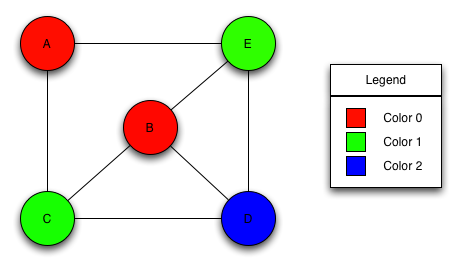
\includegraphics[scale=1]{figures/graph-sol.png}
	\caption{Lời giải của bài toán tô màu đồ thị\label{fig:graphSol}}
\end{figure}

Bài toán tô màu đồ thị yêu cầu tô màu cho các đỉnh của đồ thị sao cho không có hai đỉnh liền kề nhau có cùng màu.

Mô hình toán học:

Đồ thị $G(V,E), K$ màu cho trước \nocite{b2d1}.
\begin{itemize}
	\item $X = \{X_i | 1 \leq i \leq |V|\}$ \quad là các màu tô trên các đỉnh của đồ thị.
	\item $D = \{D_i | 1 \leq i \leq |V|\}$ \quad là miền giá trị cho các $X_i$, $D_i = \{1,\dots,K\}$
	\item Tập ràng buộc $C$:
	$X_i \neq X_j$ nếu \exists $e \in E, e = (V_i, V_j)$
	\item Hàm mục tiêu:
	Cực tiểu số lượng màu cần phải tô tren đồ thị $G(V,E)$ 
\end{itemize}

Hình \ref{fig:graphSol} là một lời giải cho bài toán tô màu đồ thị.

%----------------------------------------------------------------
\subsection{Một số kỹ thuật giải bài toán tối ưu tổ hợp}
\subsubsection*{Quy hoạch ràng buộc \cite{rossi2006handbookOfCp, pascal2005cp}}
Là kỹ thuật cơ bản để giải quyết bài toán thỏa mãn ràng buộc, mô hình của kỹ thuật quy hoạch ràng buộc như sau: 
\[ CP = Model + Search\]
Trong đó:
\begin{itemize}
	\item \textsc{Model} là tập các biến, miền giá trị và ràng buộc của bài toán.
	\item \textsc{Search} là thủ tục tìm kiếm lời giải dựa trên các ràng buộc, thủ tục này có thể là các thuật toán tìm kiếm theo chiều rộng, tìm kiếm theo chiều sâu\dots và có sử dụng các kỹ thuật cắt tỉa phù hợp làm giảm không gian tìm kiếm.
\end{itemize}

Cụ thể các bước thực hiện như sau:
\begin{itemize}
	\item Khởi tạo mô hình tìm kiếm, không cần thiết phải khởi tạo giá trị cho các biến bộ phận.
	\item Trong mỗi bước lặp, các biến bộ phận được lần lượt gán giá trị trong các thủ tục đệ quy, thủ tục này sẽ đệ quy cho đến khi tất cả các biến bộ phận được gán đầy đủ giá trị phù hợp với ràng buộc của bài toán và sẽ quay lui khi tìm được một phương án hoặc là phát hiện ra hướng tiếp theo không có phương án nào phù hợp.
\end{itemize}
Kỹ thuật này có ưu điểm dễ cài đặt, ý tưởng trong sáng tuy nhiên khi gặp bài toán có không gian lời giải lớn và rất lớn thì nó tỏ ra không hiệu quả khi không thể đưa ra được một phương án dù đó là phương án tồi vì nó yêu cầu duyệt gần như toàn bộ không gian lời giải.
\subsubsection*{Tìm kiếm cục bộ \cite{dungpq2015cbls}}
Là kỹ thuật tìm kiếm lời giải dựa trên việc lặp đi lặp lại thao tác lựa chọn lời giải có chất lượng tốt hơn trong không gian lời giải lân cận, phương pháp này có nhiều ưu điểm hơn trong những bài toán có không gian tìm kiếm lớn, cụ thể về phương pháp này tôi xin trình bày ở mục tiếp theo.
%====================================================================
\section{Tìm kiếm cục bộ dựa trên ràng buộc}
Với các bài toán tối ưu tổ hợp chúng ta luôn phải làm việc với các bộ giá trị gán cho các biến để tìm ra bộ giá trị đảm bảo thỏa mãn các ràng buộc và tối ưu hóa hàm mục tiêu. Số lượng các tập có thể của các bộ này rất lớn nên chúng ta khó có thể đưa ra một giải thuật hiệu quả để duyệt hết phương án cũng như khó có thể đưa ra một giải thuật cắt tỉa phù hợp để loại bỏ các nhánh không cần thiết.

Tiếp cận theo hướng tìm kiếm cục bộ giảm được các khó khăn nêu trên, nó không yêu cầu nhiều bộ nhớ, không yêu cầu quá nhiều thời gian tính toán. Trong tìm kiếm cục bộ ta sử dụng một số khái niệm:
\begin{itemize}
	\item \textbf{Láng giềng} của một phương án $S$ là các phương án $\{S_1, S_2,\dots, S_m\}$ được sinh ra từ $S$ bằng cách thay đổi một vài giá trị bộ phận trong phương án của $S$.
	\item \textbf{Cực tiểu địa phương} là phương án thỏa mãn các ràng buộc và có giá trị hàm mục tiêu nhỏ hơn so với các láng giềng quanh nó.
\end{itemize}

Với phương pháp tìm kiếm cục bộ, chúng ta không phải duyệt hết tất cả các bộ tổ hợp của bài toán mà thay vào đó sẽ tìm kiếm các phương án địa phương thỏa mãn các ràng buộc và cực tiểu hóa hàm mục tiêu. Từ các phương án địa phương này ta sẽ lần lượt đi đến các phương án địa phương khác tốt hơn và tiếp tục cho đến khi ta có một phương án mới là phương án tối ưu toàn cục. Sau một số bước nhất định việc tìm kiếm cục bộ sẽ đưa chúng ta đến phương án cục bộ mới tốt hơn và có thể đến được phương án tối ưu hoặc là phương án gần tối ưu mà chúng ta coi nó là chấp nhận được với yêu cầu bài toán.

Các bước của một giải thuật tìm kiếm cục bộ như sau:
\begin{itemize}
	\item \textsc{Khởi tạo:} Sinh lời giải xuất phát $s$, tính toán các vi phạm ràng buộc, hàm mục tiêu.
	\item \textsc{Tìm kiếm lân cận:} từ lời giải hiện tại, giải thuật sinh ra tập lời giải láng giềng bằng \[S = N(s)\]cách thay đổi một vài thành phần của phương án hiện tại. Từ tập lời giải mới này ta cần tìm ra phương án $s'$ có chất lượng tốt nhất.
	\item \textsc{Di chuyển:} sau khi tìm được phương án mới có chất lượng tốt, ta thực hiện di chuyển lời giải sang phương án mới này và cập nhật lại giá trị vi phạm và hàm mục tiêu.
	\item \textsc{Kiểm tra:} kiểm tra các điều kiện dừng, nếu thỏa mãn thì kết thúc tìm kiếm, nếu không sẽ thực hiện quay lại bước \textsc{Tìm kiếm lân cận}.
\end{itemize}

Các giải thuật tìm kiếm cục bộ được cải thiện đáng kể nhờ sử dụng các Heuristic để tăng cường chất lượng các lời giải láng giềng.

Giải thuật tìm kiếm cục bộ sử dụng một số phương pháp tìm kiếm sau:
\begin{itemize}
	\item Kỹ thuật leo đồi \cite{rossi2006handbookOfCp} lời giải được bắt đầu từ một vị trí ngẫu nhiên và quan sát xung quanh để xem phương án nào tốt hơn quanh nó để đi đến, sau một số lần lặp, nó sẽ đưa đến một phương án tối ưu địa phương.
	\item Kỹ thuật tìm kiếm tabu \cite{rossi2006handbookOfCp} trong bước dịch chuyển của thuật toán tìm kiếm cục bộ, một phương án được phép dịch chuyển nếu như nó hoàn toàn không bị cấm. Một phương án bị cấm là phương án đã được dịch chuyển đến trước đó. Nhờ sử dụng kỹ thuật này chúng ta giảm được sự tìm kiếm xoay vòng quanh các phương án trước đó.
\end{itemize}


%------------------------------------------------------------------
\section{Thư viện JOpenCBLS}
\subsection{Tổng quan}
JOpenCBLS là bộ thư viện được viết bằng ngôn ngữ JAVA do TS. Phạm Quang Dũng và các thành viên Lab \textsf{thuật toán và tối ưu - Viện Công nghệ thông tin truyền thông, đại học Bách Khoa Hà Nội} thiết kế và cài đặt.

Thư viện góp phần giảm công sức trong việc giải các bài toán tối ưu thỏa mãn ràng buộc bằng phương pháp tìm kiếm cục bộ. Để sử dụng hiệu quả thư viện người dùng cần biểu diễn miền giá trị, biểu diễn lời giải và các ràng buộc thích hợp. Dựa vào các thông tin được cung cấp sẵn thư viện sẽ tự động thực hiện công việc tìm kiếm kết quả theo phương pháp \textsf{tìm kiếm cục bộ}. Kiến trúc của thư viện JOpenCBLS dựa trên kiến trúc của \textsf{Constraint-based Local Search - CBLS} - \textsf{Van Hentenryck \& Michel 2005}. Thư viện được thiết kế và cài đặt trên ngôn ngữ JAVA do đó thư viện có được tính linh hoạt, tùy biến mở rộng và tái sử dụng của nền tảng JAVA. Điều đó giúp cho JOpenCBLS đã sẽ và đang góp phần rất tích cực trong quá trình giảng dạy, học tập và nghiên cứu của các cán bộ, sinh viên viện công nghệ thông tin trong Viện công nghệ thông tin - đại học Bách Khoa.

JOpenCBLS hướng đến việc đơn giản hóa các công việc xây dựng chương trình, cấu trúc dữ liệu và thiết kế thuật toán với bộ các thuật toán được cài đặt sẵn trong thư viện. Nó giúp cho người sử dụng có thêm thời gian tập trung nghiên cứu biểu diễn dữ liệu, mô hình hóa các ràng buộc của bài toán, cài đặt thử nghiệm các chiến lược tìm kiếm \textsc{heuristic} và \textsc{meta heuristic} để giải quyết bài toán.

Cấu trúc thư viện JOpenCBLS:
\begin{itemize}
	\item Mô hình (Model) nhằm mô hình hóa các bài toán, biểu diễn chúng để sau đó có thể thực hiện quá trình tìm kiếm:
	\begin{itemize}
		\item Các biến.
		\item Các đại lượng bất biến.
		\item Các hàm.
		\item Các ràng buộc.
	\end{itemize}
	\item Tìm kiếm (Search) chứa các thủ tục tìm kiếm được cài đặt sẵn với các giải thuật:
	\begin{itemize}
		\item Tabu Search.
		\item SA Search.
	\end{itemize}
\end{itemize}

%-------------------------------------------------------------------------------------------
\subsection{Các thành phần của JOpenCBLS}

\subsubsection{Mô hình}
\textbf{Biến (Variable)}
\begin{itemize}
	\item Biến trong JOpenCBLS là một đối tượng JAVA dùng để biểu diễn một bộ phận của phương án trong quá trình tìm kiếm, tập các biến cho ta một phương án.
	\item JOpenCBLS có 2 lớp cơ bản biểu diễn biến là \textsf{VarInt} và \textsf{VarIntLS}, trong đó \textsf{VarInt} là lớp biểu diễn cơ bản cho một biến, lớp \textsf{VarIntLS} kế thừa \textsf{VarInt} và cài đặt thêm các phương thức để thao tác trong quá trình tìm kiếm.
\end{itemize}

\textbf{Bất Biến (Invariants)}
\begin{itemize}
	\item Đại lượng bất biến là các đối tượng JAVA lưu giữ mối quan hệ giữa các biến, miền giá trị, mối quan hệ giữa biến và ràng buộc. Đại lượng này không thay đổi trong quá trình thực hiện tìm kiếm lời giải.
	\item Trong JOpenCBLS, \textsf{Invariant} là một \textit{interface}, nó cần được cài đặt lại khi cần thể hiện ràng buộc giữa các biến.
\end{itemize}

\textbf{Hàm (Functions)}
\begin{itemize}
	\item Là các đối tượng biểu diễn các hàm thay đổi giá trị được phụ thuộc vào giá trị các biến trong mô hình.
\end{itemize}

\textbf{Ràng buộc (Constraints)}
\begin{itemize}
	\item Là các đối tượng JAVA biểu diễn ràng buộc của bài toán, cũng giống như các hàm, nó thay đổi được giá trị và phụ thuộc vào giá trị các biến.
\end{itemize}

\subsubsection{Tìm kiếm (Search)}
JOpenCBLS có sẵn các phương thức để thao tác với biến trong quá trình tìm kiếm trong lớp \textsf{MinMaxSelector}:
\begin{itemize}
	\item \textit{MinMaxSelector(IConstraint s)}\\ là hàm khởi tạo đối tượng lựa chọn trong mô hình gắn với hệ thống ràng buộc s.
	\item \textit{selectMostViolatedVariable()}\\ là hàm trả về đối tượng biến trong mô hình có số lượng ràng buộc bị vi phạm liên quan đến nó nhiều nhất.
	\item \textit{selectMostPromissingValue(VarIntLS x)}\\ trả về giá trị làm giảm số lượng vi phạm nhiều nhất trong với biến x.
\end{itemize}

JOpenCBLS cũng đã cài đặt các kỹ thuật tìm kiếm trong lớp \textsf{TabuSearch} để giải quyết các bài toán với các thủ tục tìm kiếm tabu như:
\begin{itemize}
	\item \textit{search(s, tabuLength, maxTime, maxIter, maxStable)}\\
	Tìm kiếm với tabu heuristic nhận tham số đầu vào:
	\begin{itemize}
		\item \textit{s} Hệ thống ràng buộc.
		\item \textit{tabuLength} số bước lặp bị cấm với cùng một thao tác dịch chuyển láng giềng.
		\item \textit{maxTime} thời gian chay tối đa (tính theo giây) của thủ tục tìm kiếm tabu này.
		\item \textit{maxIter} số vòng lặp (láng giềng) tối đa trong quá trình tìm kiếm.
		\item \textit{maxStable} số lượng tối đa các láng giềng đi qua nếu không tìm thấy sự cải thiện hàm mục tiêu.
	\end{itemize}	
	\item \textit{searchAssignSwap(s, tabuLength, maxIter, maxTime)}\\
	Tìm kiếm tabu bằng cách xem xét cả việc gán giá trị cho các biến và tráo đổi giá trị từng cặp biến với nhau, nhận tham số đầu vào:
	\begin{itemize}
		\item \textit{s} hệ thống ràng buộc.
		\item \textit{tabuLength} số bước bị cấm dịch chuyển sau khi thực hiện dịch chuyển đó.
		\item \textit{maxIter} số bước lặp tối đa.
		\item \textit{maxTime} thời gian tối đa thực hiện tìm kiếm.
	\end{itemize}	
	\item \textit{searchMaintainConstraint(f, s, maxTime, maxIter, maxStable)}\\
	Tìm kiếm tabu thực hiện thỏa mãn tất cả ràng buộc trong s và cực tiểu hóa hàm mục tiêu f, nhận tham số đầu vào:
	\begin{itemize}
		\item \textit{f} hàm mục tiêu cần cực tiểu hóa.
		\item \textit{s} hệ thống ràng buộc.
		\item \textit{maxTime}  thời gian chạy tối đa của thủ tục tìm kiếm.
		\item \textit{maxIter} số lượng bước lặp tối đa.
		\item \textit{maxStable} số lần lặp tối đa để khởi động lại lời giải.
	\end{itemize}	 
\end{itemize}

\subsubsection{Ví dụ minh họa}
Dưới đây là một ví dụ minh họa việc cài đặt bài toán N-QUEENS sử dụng JOpenCBLS:
\begin{itemize}
	\item \textbf{Mô hình bài toán}
	\begin{lstlisting}
		//NQueen.java

		...		
		
		int n = 10000;
		
		LocalSearchManager ls = new LocalSearchManager();
		VarIntLS[] x = new VarIntLS[n];
		
		for (int i = 0; i < n; i++){
			x[i] = new VarIntLS(ls, 0, n - 1);
			
		ConstraintSystem s = new ConstraintSystem(ls);
		s.post(new AllDifferent(x));
		
		IFunction[] f1 = new IFunction[n];
		for (int i = 0; i < n; i++)
			f1[i] = new FuncPlus(x[i], i);
		s.post(new AllDifferent(f1));
		
		IFunction[] f2 = new IFunction[n];
		for (int i = 0; i < n; i++)
			f2[i] = new FuncPlus(x[i], -i);
		s.post(new AllDifferent(f2));
		
		ls.close();		
		...
	\end{lstlisting}
	Để thực hiện khởi tạo chúng ta cần khai báo một \textsf{LocalSearchManager} quả lý tất cả các biến, sau đó khai báo các biến trong mô hình và khởi tạo nó. Tiếp theo chúng ta cần có một hệ thống ràng buộc và thực hiện lưu giữ các ràng buộc lại trong hệ thống ràng buộc $s$. Ở đây, với bài toán n-queens chúng ta có 3 ràng buộc cơ bản:
	\begin{itemize}
		\item các quân hậu không cùng nằm trên cùng một cột,
		\item các quân hậu không cùng nằm trên cùng một đường chéo thuận,
		\item các quân hậu không cùng nằm trên cùng một đường chéo ngược. 
	\end{itemize}
	Sau khi khởi tạo các biến, mô hình và tải các ràng buộc, chúng ta cần đóng mô hình để thư viện thực hiện các thủ tục khởi tạo, cập nhật hệ thống ràng buộc cần thiết.
	\item \textbf{Thực hiện tìm kiếm}
	\begin{lstlisting}
		//NQueen.java
		MinMaxSelector mms = new MinMaxSelector(s);
		int it = 0;
		while(it < 10000 && s.violations() > 0){
			VarIntLS variable = mms.selectMostViolatedVariable();
			int selectValue = mms.selectMostPromissingValue(variable);
			variable.setValuePropagate(selectValue);
			it++;
		}
		System.out.println("Current violations: " + s.violation());
	\end{lstlisting}
	Với đoạn mã thực hiện việc tìm kiếm này chúng ta có một đối tượng lựa chọn để lấy các thông tin, các đối tượng mà chúng ta yêu cầu sau đó tiếp tục thực hiện gán giá trị cho các biến chúng ta lấy được. Cụ thể ở đây ta luôn chọn đối tượng biến có số lượng vi phạm có liên quan đến nó là nhiều nhất sau đó gán cho nó giá trị mới sao cho số lượng vi phảm được giảm đi cũng là nhiều nhất, tiếp tục lặp thao tác vừa rồi cho tới khi không còn vi phạm hoặc số vòng lặp vượt quá tối đa. Kết thúc vòng lặp chúng ta có kết quả của thủ tục tìm kiếm này.
\end{itemize}

%============================================================================================
%\section{Kết luận}
%Các bài toán tối ưu tổ hợp rất phổ biến trong cuộc sống và cũng là những vấn đề lớn cần giải quyết song không phải dễ dàng giải quyết chúng, công việc giải quyết đòi hỏi rất nhiều thời gian và công sức.

%Tìm kiếm cục bộ dựa trên ràng buộc là phương pháp khả thi hơn cả và với thư viện JOpenCBLS của tiến sỹ Phạm Quang Dũng chúng ta có một bộ công cụ đủ mạnh để thực hiện các bài toán này. Trong phần tiếp theo tôi sẽ đi sâu phân tích, mô hình và giải quyết một bài toán trong số các bài toán tối ưu này đó là bài toán \textsc{đóng thùng} (Bin Packing) ở mức 2 chiều.

    \chapter{Bài Toán Đóng Thùng 2D - Bin Packing 2D}
\label{chap:binPacking}
%============================================================================
\section{Phát biểu bài toán}
Trong thực tế cuộc sống chúng ta rât hay gặp phải vấn đề cần giải quyết: liệu có thể xếp tất cả những vật này vào cái túi này, cái hộp này hay cái thùng kia không, lựa chọn cái nào phù hợp để vừa chứa đủ những thứ này? Các yêu cầu này nằm trong lớp bài toán đóng thùng \cite{hopper2000twodimensional}.

Để mô hình hóa tốt hơn tôi sẽ xét bài toán này trong không gian 2 chiều, khi đó các vật phẩm chỉ còn lại kích thước rộng ($w_i$) và cao $(h_i)$, và thùng có kích thước $ W \times H $. Như vậy chúng ta có bài toán đóng thùng 2 chiều (Bin Packing 2D) với phát biểu như sau:\\
Cho trước một cái thùng với kích thước $W \times H$ và $N$ vật phẩm $\{X_1,\dots,X_n\}$, các vật phẩm $X_i$ có kích thước tương ứng là $w_i \times h_i$ ($1 \leq i \leq N$). Ta cần đặt các vật phẩm (có thể xoay theo chiều ngang hoặc dọc) này vào các vị trí trong thùng sao cho các vật không chồng lấn lên nhau, không vượt khỏi biên của thùng đã cho. Câu hỏi đặt ra là liệu có một phương án sắp xếp nào đó thỏa mãn yêu cầu trên không và nếu có hãy đưa ra phương án sắp xếp đó.

%============================================================================
\section{Mô hình toán học}

\subsection*{Mô hình cơ bản}

Cho trước một cái thùng với kích thước $(W \times H)$ và $N$ vật với kích thước tương ứng được cho bởi: $(w_1, h_1),\dots,(w_n, h_n)$.\\
\textbf{Với các biến:}
\begin{align*}
	X_i &\in \{0,\dots,W-1\} \quad &1 \leq i \leq N \\
	Y_i &\in \{0,\dots,H-1\} \quad &1 \leq i \leq N \\
	R_i &\in \{0,1\} \quad &1 \leq i \leq N
\end{align*}
Các kích thước và tọa độ vật phẩm như hình ~\ref{fig:itemPositions} trong đó:
\begin{description}
	\item[$X_i$] là tọa độ theo phương ngang đặt vật thứ $i$ trong thùng.
	\item[$Y_i$] là tọa độ theo phương dọc đặt vật thứ $i$ trong thùng.
	\item[$R_i$] xác định vật phẩm được xoay hoặc không.
\end{description}

\begin{figure}[H]
	\centering
	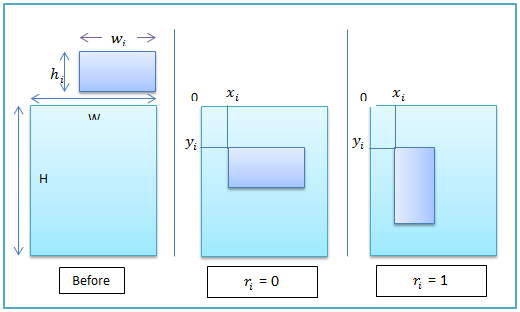
\includegraphics[scale=1]{figures/items-pos.png}
	\caption{Kích thước và tọa độ các vật phẩm\label{fig:itemPositions}}
\end{figure}

\textbf{Thỏa mãn các ràng buộc:}
\begin{align}
	C_1 &: 
	\begin{cases}
		X_i + w_i \leq W &\text{nếu } R_i = 0 \\
		X_i + h_i \leq W &\text{nếu } R_i = 1
	\end{cases}
	\\
	C_2 &: 
	\begin{cases}
		Y_i + h_i \leq H &\text{nếu } R_i = 0 \\
		Y_i + w_i \leq H &\text{nếu } R_i = 1
	\end{cases}
	\\
	C_3 &: 
	\begin{cases}
		X_i + w_i \leq X_j || X_j + w_j \leq X_i || Y_i + h_i \leq Y_j || Y_j + h_j \leq Y_i &\text{nếu }R_i = 0, R_j = 0 \\ 
		X_i + w_i \leq X_j || X_j + h_j \leq X_i || Y_i + h_i \leq Y_j || Y_j + w_j \leq Y_i &\text{nếu }R_i = 0, R_j = 1 \\ 
		X_i + h_i \leq X_j || X_j + w_j \leq X_i || Y_i + w_i \leq Y_j || Y_j + h_j \leq Y_i &\text{nếu }R_i = 1, R_j = 0 \\ 
		X_i + h_i \leq X_j || X_j + h_j \leq X_i || Y_i + w_i \leq Y_j || Y_j + w_j \leq Y_i &\text{nếu }R_i = 1, R_j = 1
	\end{cases}
\end{align}
Với:
\begin{description}
	\item[$C_1$] là ràng buộc các vật phẩm không được vượt quá biên rộng của thùng.
	\item[$C_2$] là ràng buộc các vật phẩm không được vượt quá biên cao của thùng.
	\item[$C_3$] là ràng buộc mọi vật phẩm không chồng lấn lên nhau.
\end{description}

\subsection*{Mô hình mở rộng}
Ở mô hình trước chúng ta có ba mảng chứa các biến là $X$, $Y$ và $R$, để thực hiện tìm kiếm trong mô hình tốt hơn chúng tôi đề xuất thực hiện việc gắn các biến tọa độ $x$ và $y$ với nhau thông qua một biến $pos$. Biến $pos$ này sẽ bao gồm thông tin của hai biến $x$ và $y$ như sau:
\begin{align}
	pos = y \times W + x
\end{align}
với 
\begin{itemize}
	\item[$pos$] là biến chứa thông tin tọa độ của vật trong thùng.
	\item[$x$] là biến tọa độ theo phương ngang trong thùng như ở mô hình trước.
	\item[$y$] là biến tọa độ theo phương dọc trong thùng như mô hình trước.
	\item[$W$] là chiều rộng của thùng.
\end{itemize}
Từ tọa độ $pos$ chúng ta có thể tính toán được tọa độ của các vật như sau:
\begin{align}
	\begin{cases}
		x = pos _{mode W}\\
		y = pos / W
	\end{cases}
\end{align}
%============================================================================
\section{Ứng dụng}
Bài toán đóng thùng có ứng dụng rộng rãi trong đóng gói, vận chuyển và bố trí linh kiện.
\begin{itemize}
	\item Các hãng vận chuyển thường phải xếp các vật phẩm vào các container, kích thước container là cố định nên yêu cầu cần phải xếp sao cho tiết kiệm diện tích nhất số lượng các vật phẩm cần vận chuyển.
	\item Các công ty chuyển phát nhanh cần đóng gói các gói hàng trước khi đưa lên máy bay, kích thước cho phép trên máy bay là giới hạn nên yêu cầu cần phải sắp xếp một cách tiết kiệm nhất.
	\item Phân chia các khu vực bố trí linh kiện điện tử cũng rất quan trọng bên cạnh việc nghiên cứu làm giảm kích thước linh kiện khi các thiết bị ngày nay yêu cầu nhỏ gọn mà vẫn đảm bảo hiệu năng cao, an toàn cho người sử dụng.
	\item $\dots$
\end{itemize}

    \chapter{Áp dụng thư viện JOpenCBLS vào bài toán BP2D}
\label{chap:implement}
Trong chương này tôi sẽ trình bày cách cài đặt thuật toán tìm kiếm cục bộ dựa trên ràng buộc vào bài toán đóng thùng 2d đã được trình bày ở chương \ref{chap:binPacking}.

%-----------------------------------------------------------------------
\section{Các chức năng cài đặt thêm}
Để cài đặt với mô hình mở rộng của bài toán đóng thùng 2D đã trình bày ở mục trước, chúng tôi đề xuất cài đặt thêm một số lớp có các chức năng sau:
\subsection{Phép chia nguyên (Function)}
Phép chia nguyên là phép toán được định nghĩa trên vành số nguyên, nó bao gồm hai toán tử là toán tử chia và toán tử bị chia. Trong bài toán BP2D tôi chỉ thao tác chính trên số nguyên nên việc sử dụng thêm phép chia nguyên là cần thiết. Cụ thể trong BP2D để gắn liền tọa độ theo phương $x$ và theo phương $y$ của vật phẩm tôi sử dụng một biến trong mô hình lưu giữ một đại lượng 
\[ posCombine_i = x_i \times W + y_i \quad 1 \leq i \leq N \]
Nó cho phép chúng ta có thêm nhiều láng giềng hơn trong quá trình duyệt tìm kiếm. Việc lấy giá trị tọa độ $y_i$ được thực hiện đơn giản bằng một phép chia nguyên.

Phép chia nguyên được cài đặt bởi lớp \textsf{Devide} là một định nghĩa hàm, nó nhận khởi tạo là một biến và một số nguyên cố định. Giá trị của hàm này chỉ phụ thuộc vào giá trị của biến tham số truyền vào hàm khởi tạo.
\begin{lstlisting}
	// Divide.java
	...
	public Divide(VarIntLS var, int mod) {
		this.variable = var;
		this.mod = mod;
		
		this.manager = var.getLocalSearchManager();
		
		manager.post(this);
	}
	...
\end{lstlisting}
trong đó:
\begin{itemize}
	\item \textit{var} là tham chiếu đến đối tượng \textsf{VarIntLS} chứa giá trị bị chia.
	\item \textit{mod} là số nguyên chứa giá trị số chia.
\end{itemize}
\subsection{Phép lấy phần dư (Function)}
Bên cạnh phép chia nguyên là phép lấy phần dư (module) cũng được định nghĩa trên vành số nguyên gồm hai toán tử là toán tử lấy mô-đun và toán tử mô-đun. Trong BP2D tôi sử dụng toán tử này để lấy lại giá trị tọa độ $x_i$ của vật phẩm trong túi từ đại lượng $posCombine_i$.

Phép lấy phần dư được cài đặt bởi lớp \textsf{Module} là một định nghĩa hàm, nhận khởi tạo là một biến và một số nguyên cố định, giá trị của hàm này là kết quả phép chia lấy phần dư của giá trị biến truyền vào và số nguyên đó.

\begin{lstlisting}
	// Module.java
	...
	public Module(VarIntLS var, int mod) {
		this.variable = var;
		this.mod = mod;
		
		this.manager = var.getLocalSearchManager();
		manager.post(this);
	}
	
	...
\end{lstlisting}
trong đó:
\begin{itemize}
	\item \textit{var} là tham chiếu đến đối tượng \textsf{VarIntLS} chứa giá trị lấy phần dư.
	\item \textit{mod} là số nguyên chứa giá trị số chia.
\end{itemize}
\subsection{Các lớp có chức năng tìm kiếm}
Ngoài các lớp có sẵn trong thư viện JOpenCBLS tôi có cài đặt thử nghiệm thêm các lớp thực hiện các phương thức tìm kiếm khác nhau nhằm phù hợp hơn với mô hình và kiến trúc của ứng dụng.
\subsubsection{Tabu Search}
Tabu search là một kỹ thuật sử dụng phổ biến và rất hiệu quả trong các bài toán tìm kiếm cục bộ, ở đây tôi cài đặt các lớp thực hiện các công việc tìm kiếm \textit{tabu} trong các mô hình của JOpenCBLS. Các lớp tìm kiếm này sẽ cài đặt một \textit{interface} là \textsf{SearchMethod} chứa các phương thức điều khiển:
\begin{itemize}
	\item \textit{run()} sẽ bắt đầu quá trình tìm kiếm.
	\item \textit{stop()} sẽ kết thúc tiến trình tìm kiếm hiện tại.
\end{itemize}
Khi bắt đầu một tiến trình tìm kiếm thông thường các lớp sẽ gọi phương thức tìm kiếm tương ứng của mình đã được cài đặt:
\begin{itemize}
	\item \textsf{SearchTabuAssign} là lớp cài đặt phương thức tìm kiếm tabu bằng cách xem xét láng giềng là các bộ tổ hợp mới có được từ bộ tổ hợp cũ bằng cách thay đổi duy nhất một thành phần trong nó. Đối tượng của lớp này sẽ thực hiện tìm kiếm trong phương thức \textit{searchAssign()}.
	\item \textsf{SearchTabuSwap} là lớp cài đặt phương thức tìm kiếm tabu bằng cách xem xét láng giềng là các bộ tổ hợp mới có được bằng cách tráo đổi giá trị của đúng 2 thành phần trong bộ tổ hợp cũ. Đối tượng của lớp này sẽ thực hiện tìm kiếm trong phương thức \textit{searchSwap()}.
	\item \textsf{SearchTabuMixAssignSwap} là lớp cài đặt phương thức tìm kiếm tabu bằng cách xem xét láng giềng là hợp của các láng giềng trong tìm kiếm với \textsf{SearchTabuAssign} và \textsf{SearchTabuSwap}. Đối tượng của lớp này sẽ thực hiện tìm kiếm trong phương thức \textit{searchMix()}.
\end{itemize}

Mỗi lớp tìm kiếm này có thể chạy độc lập trong môi trường đa luồng, chúng ta có thể khởi tạo nó bằng một luồng mới và thực thi công việc tìm kiếm độc lập, việc này giúp cho phần ứng dụng trở nên thông suốt hơn. Các tiến trình mới này có thể bị hủy trước khi hoàn thành công việc tìm kiếm nếu như chúng ta gọi thủ tục kết thúc (\textit{stop()}) từ một tiến trình khác.

\subsubsection{Random Search}
Lớp \textsf{RandomSearch} là một lớp có chức năng tìm kiếm với phương thức tìm kiếm ngẫu nhiên, lớp này cài đặt với mục đích thử nghiệm.
%-----------------------------------------------------------------------
\section{Dữ liệu và mô hình hóa}
Mô hình của bài toán được đặt hoàn toàn trong lớp \textsf{BpModelCombine}, nó kế thừa một \textit{interface} là \textsf{SearchModel}, cài đặt \textit{interface} này cho phép các phương thức tìm kiếm ở trên có thể sử dụng model này trong quá trình tìm kiếm, tạo sự độc lập giữa cài đặt phương thức tìm kiếm và cài đặt mô hình.

\subsection{Dữ liệu}
Trong lớp \textsf{BpModelCombine} bao gồm:
\begin{itemize}
	\item \textbf{Các thuộc tính}
	\begin{lstlisting}
		//BpModelCombine.java
		private LocalSearchManager manager;
		private ConstraintSystem cs;
	
		private SearchEventPool pool;
	
		private BpData data;
		private int itemCount;
		private int binWidth;
		private int binHeight;
		private int[] itemWidths;
		private int[] itemHeights;
	
	\end{lstlisting}

	Có tác dụng như sau:
	\begin{itemize}
		\item \textit{manager} là đối tượng quản lý toàn bộ mô hình.
		\item \textit{cs} là đối tượng quản lý hệ thống ràng buộc.
		\item \textit{pool} là đối tượng giữ lại các mốc trong quá trình tìm kiếm.
		\item \textit{data} là đối tượng chịu trách nhiệm đọc dữ liệu từ tệp tin và trích xuất ra các thông tin cần thiết.
		\item \textit{itemCount} là số lượng vật phẩm ($N$).
		\item \textit{binWidth} là chiều rộng của thùng ($W$).
		\item \textit{binHeight} là chiều cao của thùng ($H$).
		\item \textit{itemWidths} là mảng lưu trữ chiều rộng của các vật phẩm: $[w_1,\dotsc,w_N]$.
		\item \textit{itemHeights} là mảng lưu trữ chiều cao của các vật phẩm: $[h_1,\dotsc,h_N]$.
	\end{itemize}

	\item \textbf{Biến mô hình}
	\begin{lstlisting}
		//BpModelCombine.java
	
		private VarIntLS[] combinedPos;
		private VarIntLS[] rotated;
		
	\end{lstlisting}
	có tác dụng:
	\begin{itemize}
		\item \textit{combinedPos} là đối tượng lưu giữ giá trị thể hiện vị trí của vật phẩm trong thùng như đã trình bày ở mục trước: \[combinedPos[i] = Y_i \times W + X_i \quad \text{với } 1 \leq i \leq N\]
		\item \textit{rotated} là đối tượng lưu giữ trạng thái hiện thời của vật phẩm: được xoay hay không được xoay.
		\[		
		\begin{cases}
			rotated[i] = 1 \quad \text{nếu vật thứ $i$ đã được xoay} \\
			rotated[i] = 0 \quad \text{nếu vật thứ $i$ không được xoay}
		\end{cases}
		\]
	\end{itemize}
\end{itemize}

\subsection{Mô hình}
\subsubsection{Khai báo và cấp phát bộ nhớ}
	Các thao tác khai báo và cấp phát bộ nhớ được thực hiện trong phạm vi của thủ tục:
	\begin{lstlisting}
		//BpModelCombine.java
		...
		private void allocateVariable(){
			final int COMBINE_MAX = (binWidth - 1) * binHeight;
			combinedPos = new VarIntLS[itemCount];
			rotated = new VarIntLS[itemCount];
			for(int i = 0; i< itemCount; i++){
				combinedPos[i] = new VarIntLS(manager, 0, COMBINE_MAX - 1);
				rotated[i] = new VarIntLS(manager, 0, 1);
			}
		}
		...
	\end{lstlisting}
	bao gồm:
	\begin{itemize}
		\item khai báo và khởi tạo giá trị cho các phần tử của mảng $combinedPos$,
		\item khai báo và khởi tạo giá trị cho các phần tử của mảng $rotated$.
	\end{itemize}

\subsubsection{Tải các ràng buộc}
	Thao tác khai báo các ràng buộc được thực hiện trong thủ tục \textit{loadConstraints()}:
	\begin{itemize}
		\item Tính toán vị trí tọa độ $x, y$:
		\begin{lstlisting}
		
		// Calculate x position and y position of all items
		IFunction[] left = new IFunction[itemCount];
		IFunction[] top = new IFunction[itemCount];
		for(int i = 0; i< itemCount; i++){
			left[i] = new Module(combinedPos[i], binWidth);
			top[i] = new Divide(combinedPos[i], binWidth);
		}
		
		\end{lstlisting}
		\item Tính toán tọa độ biên của các hộp trong thùng:
		
		\begin{lstlisting}
		
		// Calculate bound of all item
		IFunction[] right = new IFunction[itemCount];
		IFunction[] bottom = new IFunction[itemCount];
		IFunction[] rightRot = new IFunction[itemCount];
		IFunction[] bottomRot = new IFunction[itemCount];
		for(int i = 0; i< itemCount; i++){
			right[i] = new FuncPlus(left[i], itemWidths[i]);
			bottom[i] = new FuncPlus(top[i], itemHeights[i]);
			rightRot[i] = new FuncPlus(left[i], itemHeights[i]);
			bottomRot[i] = new FuncPlus(top[i], itemWidths[i]);
		}
		\end{lstlisting}
		\item Tải ràng buộc không chồng lấn giữa các vật:
		\begin{lstlisting}
		
		// All items must not overlap
		for(int i = 0; i< itemCount; i++){
			for(int j = i + 1; j< itemCount; j++){
				IConstraint[] allCase = new IConstraint[4];
				// Case 0 item 1 NOT rotated, item 2 NOT rotated
				IConstraint[] tmp = new IConstraint[4];
				tmp[0] = new LessOrEqual(right[i], left[j]);
				tmp[1] = new LessOrEqual(right[j], left[i]);
				tmp[2] = new LessOrEqual(bottom[i], top[j]);
				tmp[3] = new LessOrEqual(bottom[j], top[i]);
				IConstraint[] tmpCase = new IConstraint[3];
				tmpCase[0] = new OR(tmp);
				tmpCase[1] = new IsEqual(rotated[i], 0);
				tmpCase[2] = new IsEqual(rotated[j], 0);
				allCase[0] = new AND(tmpCase);
				// Case 1 item 1 NOT rotated, item 2 rotated
				...
				allCase[1] = new AND(tmpCase);
				// Case 2 item 1 rotated, item 2 NOT rotated
				...
				allCase[2] = new AND(tmpCase);
				// Case 3 item 1 rotated, item 2 rotated
				tmp = new IConstraint[4];
				...
				allCase[3] = new AND(tmpCase);
				
				// Combine all case
				cs.post(new OR(allCase));
			}
		}
		
		\end{lstlisting}
		
		\item Tải ràng buộc vật phẩm không vượt quá phạm vi của thùng:
		\begin{lstlisting}
		
		// All items must be not overlap with bin-bound
		for(int i = 0; i< itemCount; i++){
			IConstraint[] allCase = new IConstraint[2];
			// Case 0 : item NOT rotated
			IConstraint[] tmp = new IConstraint[3];
			tmp[0] = new LessOrEqual(right[i], binWidth);
			tmp[1] = new LessOrEqual(bottom[i], binHeight);
			tmp[2] = new IsEqual(rotated[i], 0);
			allCase[0] = new AND(tmp);
			// Case 1 : item rotated
			tmp = new IConstraint[3];
			tmp[0] = new LessOrEqual(rightRot[i], binWidth);
			tmp[1] = new LessOrEqual(bottomRot[i], binHeight);
			tmp[2] = new IsEqual(rotated[i], 1);
			allCase[1] = new AND(tmp);
			
			// Combine all case
			cs.post(new OR(allCase));
		}
		
		\end{lstlisting}
		
	\end{itemize}
	
\subsubsection{Thực hiện tìm kiếm}
Chúng ta sẽ thực hiện tìm kiếm cục bộ bằng cách: sử dụng một đối tượng tìm kiếm (\textsf{SearchTabuSwap}, \textsf{RandomSearch},$\dots$) khởi tạo với mô hình vừa được khai báo gọi thủ tục \textit{run()}.


    \chapter{Chương Trình Minh Họa}
\label{chap:presentation}

%==================================================================
\section{Mô hình chương trình}
Chương trình minh họa được cài đặt trên môi trường ứng dụng WEB sử dụng các công nghệ \textbf{Servlet, Bootstrap, Javascript AngularJS}.
%--------------------------------------------------------------
\subsection{Tổng Quan}
\begin{figure}
	\centering
	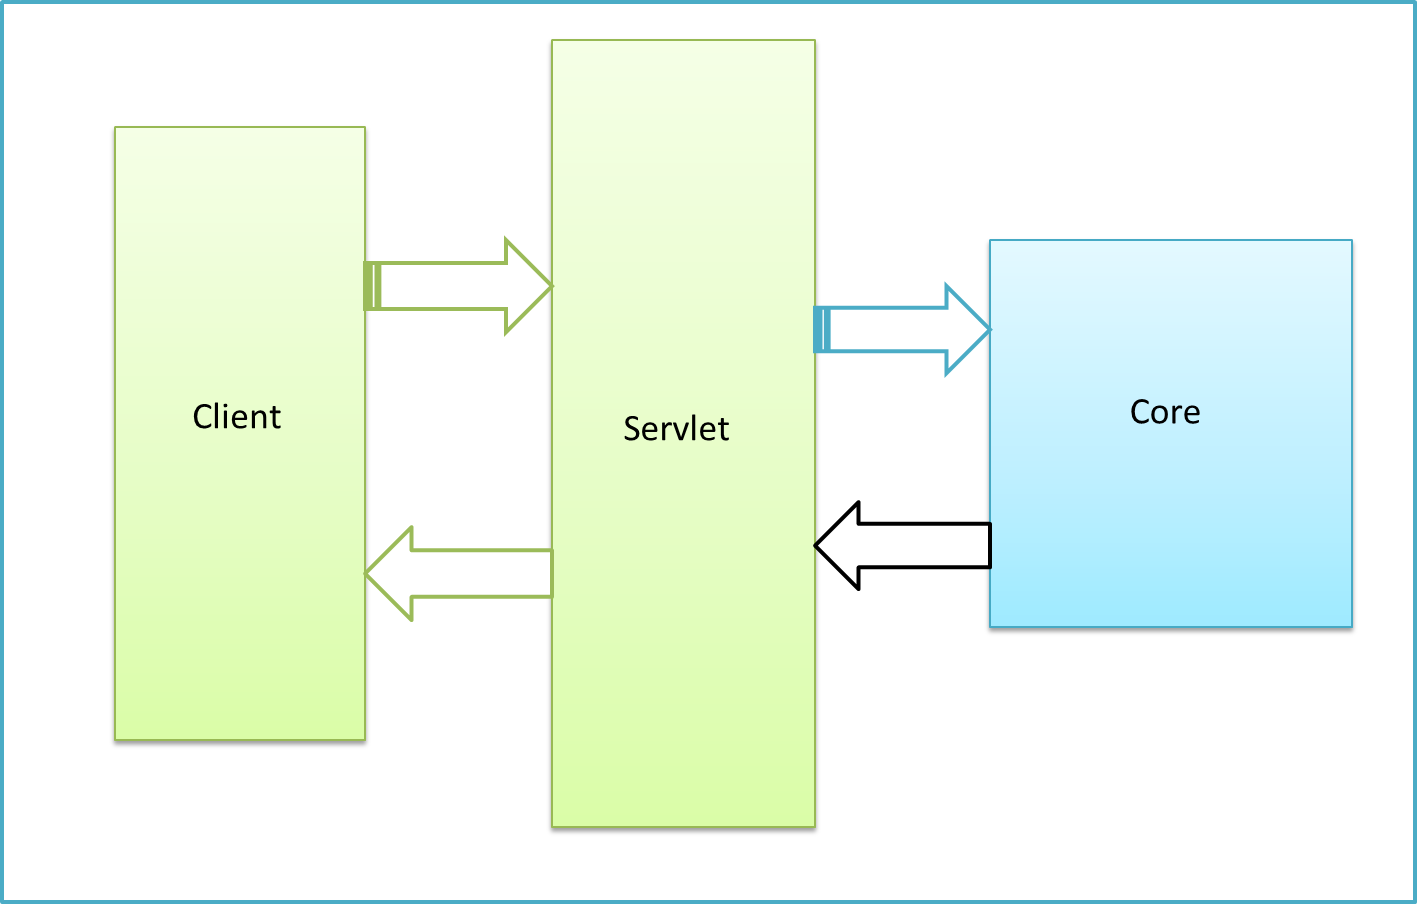
\includegraphics[scale=0.5]{figures/app-overview.png}
	\caption{Kiến trúc tổng quan ứng dụng \label{fig:appOverview}}
\end{figure}

Hình \ref{fig:appOverview} mô tả kiến trúc tổng quan của ứng dụng web cho bài toán đóng thùng 2D, chương trình gồm 3 phần:
\begin{itemize}
	\item \textbf{Core} chứa các lớp xử lý nghiệp vụ của bài toán đóng thùng, bao gồm đọc ghi dữ liệu, mô hình hóa và thực hiện tìm kiếm.
	\item \textbf{Servlet} chứa các lớp xử lý yêu cầu từ phía trình duyệt web của người dùng, nó xử lý các thao tác điều khiển của người dùng và cũng là nơi trả lại các thông tin cần thiết về cho client.
	\item \textbf{Client} là ứng dụng ở phía người dùng xử lý các thông tin trả về từ servlet và hiển trị lên màn hình trình duyệt web.
\end{itemize}
Cụ thể các phần của chương trình như sau:
%--------------------------------------------------------------
\subsection{Server}
\subsubsection{Core}
Phần \textbf{Core} bao gồm:
\begin{itemize}
	\item Các lớp xử lý việc đọc dữ liệu từ hệ thống tệp tin của Server, các lớp này nằm trong gói \textit{binpacking.io}
	\begin{itemize}
		\item \textsf{BpData} chứa các thông tin của tệp tin dữ liệu, mỗi đối tượng của lớp này chứa đầy đủ thông tin của một tệp tin dữ liệu của BP2D: tệp tin (\textit{file}), chiều rộng thùng (\textit{binWidth}), chiều cao thùng (\textit{binHeight}), số lượng vật phẩm (\textit{itemCount}), chiều rộng các vật phẩm (\textit{itemHeights}), chiều cao các vậy phẩm (\textit{itemHeights}). Ngoài ra các đối tượng của lớp này chỉ thực sự đọc dữ liệu khi cần thiết, điều này giúp cải thiện hiệu năng hệ thống, tiết kiệm tài nguyên máy chủ.
		\begin{lstlisting}
		//BpData.java
		
		private File file;
		private boolean isReady;
		private int binWidth;
		private int binHeight;
		private int itemCount;
	
		private int[] itemWidths;
		private int[] itemHeights;
		
		\end{lstlisting}
		\item \textsc{BpDataManager} quản lý toàn bộ các đối tượng \textsf{BpData}, bảo đảm mỗi đối tượng \textsf{BpData} luôn chỉ cần khởi tạo một lần và có thể sử dụng cho nhiều mô hình khác nhau. Đối tượng của lớp này sẽ là nơi cung cấp dữ liệu cho các lớp yêu cầu xử lý mô hình, tìm kiếm\dots.
	\end{itemize}
	\item Lớp mô hình hóa cho bài toán \textsf{BpModelCombine} nằm trong gói \textit{binpacking2d.model} có tác dụng mô hình bài toán đóng thùng vào thư viện JOpenCBLS.
	\item Các lớp khởi tạo phương án bắt đầu cho bài toán, mỗi lớp khởi tạo sẽ có một cách thức khởi tạo riêng cho các mô hình tương ứng. Với bài toán BP2D có các cách khởi tạo tương ứng với các lớp:
	\begin{itemize}
		\item \textsf{BpAllZeroInitMethod} khởi tạo phương án bằng cách xếp tất cả các vật phẩm vào vị trí góc của thùng và không có vật phẩm nào được xoay.
		\item \textsf{BpRandomInitMethod} khởi tạo một cách ngẫu nhiên vị trí các vật phẩm, chúng cũng có thể được xoay hoặc không và hoàn toàn ngẫu nhiên.
	\end{itemize}
	Ngoài ra các đối tượng của các lớp khởi tạo này cũng được quản lý bởi đối tượng của lớp \textsf{BpInitMethodManager}, đối tượng này sẽ chỉ cho hệ thống những lớp khởi tạo nào được phép sử dụng và khởi tạo sẵn các lớp khởi tạo.
	\item Chương trình còn cài đặt thêm một số lớp có chức năng tương tự như trong thư viện JOpenCBLS có tác dụng thử nghiệm và phù hợp hơn với chương trình đa luồng.
\end{itemize}

\subsubsection{Servlet}
Các Servlet là các lớp nằm trong gói \textit{binpacking2d.servlet} có vai trò giao tiếp với client, bao gồm:
\begin{itemize}
	\item \textbf{control - ControlServlet} là Servlet chịu trách nhiệm nhận các thông điệp điều khiển từ phía người dùng sau đó nó tương tác với phần Core để thực hiện các tác vụ này. \textsf{ControlServlet} xử lý các thông điệp từ các phương thức GET của http:
	\begin{itemize}
		\item \textit{control?action=init{\&}initMode=<modeId>{\&}fileId=<fileId>} khởi tạo mô hình bằng chỉ số của thủ tục tìm kiếm và chỉ số của tệp tin trên hệ thống, các chỉ số định danh này được cố định và được cung cấp bởi các quản lý tương ứng: \textsc{SearchMethodManager, BpDataManager}.
		\item \textit{control?action=start} bắt đầu tiến trình tìm kiếm cục bộ đã được khởi tạo trước đó, nếu chưa được khởi tạo trước thì thao tác này sẽ không thực hiện tìm kiếm.
		\item \textit{action=stop} sẽ dừng tiến trình tìm kiếm đang thực thi trên máy chủ.
	\end{itemize}
	\item \textbf{events - EventsServlet} sẽ liệt kê tất cả các sự kiện diễn ra trên máy chủ trong quá trình tìm kiếm, các sự kiện được trả dưới dạng JSON cấu trúc như sau: 
		\begin{lstlisting}
		{
			"state": {
				"running": RUNNING_VALUE,
				"ready": READY_VALUE
			}
			"events":[
				{
					"violations": VIOLATION,
					"name": EVENT_NAME,
					"items": LIST_ITEMS
				},
				...
			]
		}
		\end{lstlisting}
	
	\item \textbf{fetch - ResourceServlet} là Servlet chịu trách nhiệm xử lý các yêu cầu lấy thông tin tài nguyên từ người dùng, nó cung cấp các loại tài nguyên:
	\begin{itemize}
		\item \textit{fetch?res=files} khi nhận được yêu cầu này nó sẽ trả về dưới dạng JSON các tệp tin dữ liệu của bài toán BP2D đang có trên thư mục dữ liệu của máy chủ. Thông điệp trả về sẽ có dạng JSON:
		\begin{lstlisting}
		[
			{		
				"name": FILE_NAME,
				"id" : FILE_ID
			},
			...
		]
		\end{lstlisting}
		\item \textit{fetch?res=search} cung cấp các thuật toán tìm kiếm đã được cài đặt trong ứng dụng của máy chủ, thông tin trả về dưới dạng JSON:
		\begin{lstlisting}
		[
			SEARCH_METHOD,
			...
		]
		\end{lstlisting}
		\item \textit{fetch?res=init} cung cấp các thuật toán khởi tạo dưới dạng JSON:
		\begin{lstlisting}
		[
			INIT_METHOD,
			...
		]
		\end{lstlisting}
	\end{itemize}
\end{itemize}

%--------------------------------------------------------------
\subsection{Client}
Chương trình phía client được cài đặt sử dụng công nghệ AngularJS và Bootstrap:
\begin{itemize}
	\item \textsc{AngularJS} là một framework javascript được phát triển bởi các kỹ sư của Google, nó thay đổi cách các lập trình viên làm việc với javascript, cung cấp các cách thức lập trình nhanh, logic, hiệu quả trên các ứng dụng web.
	\item \textsc{Bootstrap3} là một thư viện css3 nhằm làm cho việc thiết kế các trang web trở nên đơn giản, chuẩn mực.
\end{itemize}

Trong ứng dụng phía client của bài toán BP2D sử dụng các thành phần:
\begin{itemize}
	\item \textit{bin.js} định nghĩa chỉ thị của AngularJS, khi nó được khai báo trên html canvas, nó sẽ vẽ ra hình ảnh để mô tả vị trí của các vật phẩm trong thùng, nếu các vật chồng lấn lên nhau nó sẽ thông báo bằng cách vẽ viền của nó màu đỏ.
	\item \textit{poller.js} khai báo một dịch vụ mới trên AngularJS, dịch vụ này được AngularJS thực thi khi khởi tạo và nó được thực thi trong suốt quá trình ứng dụng phía client được mở. Khi được hoạt động, nó sẽ định kỳ lấy các sự kiện từ trên máy chủ về và dùng các hàm xử lý được khai báo trước để xử lý các dữ liệu sự kiện này. Thông thường các hàm xử lý sẽ cập nhật hiển thị các vật nằm trong thùng.
	\item \textit{index.js} định nghĩa ứng dụng AngularJS, thiết lập các hàm xử lý sự kiện cho \textit{poller} và thực hiện các thao tác khởi tạo cần thiết.
	\item \textit{index.html} là trang html chính của ứng dụng BP2D, nó GET từ Server và được cập nhật liên tục khi các sự kiện xảy ra.
\end{itemize}
%--------------------------------------------------------------
\subsection{Giao tiếp}
Khi máy chủ tiếp nhận một yêu cầu từ phía client, nó sẽ gửi về tệp tin \textit{index.html} cho client để thực thi trên trình duyệt web. Khi bắt đầu ứng dụng web phía client sẽ thực hiện lấy các thông tin tài nguyên từ máy chủ như các tệp tin, các thủ tục khởi tạo, các thuật toán tìm kiếm và đồng thời nó cũng yêu cầu máy chủ khởi tạo sẵn với một số tham số mặc định. Với ứng dụng web phía client này, người dùng có thể thực hiện các thao tác:
\begin{itemize}
	\item Lựa chọn tệp tin dữ liệu: ứng dụng cho phép người dùng lựa chọn tệp tin dữ liệu thông qua bảng chọn. Khi người dùng lựa chọn xong tệp tin dữ liệu, client sẽ yêu cầu server thực hiện luôn thao tác khởi tạo tương ứng.
	\item Lựa chọn thủ tục khởi tạo: khi người dùng thay đổi thủ tục khởi tạo chương trình cũng sẽ tự động gửi yêu cầu khởi tạo lên server và tự động cập nhật trạng thái lên màn hình.
	\item Lựa chọn thuật toán tìm kiếm: chương trình cung cấp nhiều lựa chọn tìm kiếm cho bài toán, các thuật toán được cài đặt một cách tổng quát và có thể dùng cho nhiều mô hình.
	\item Bắt đầu tìm kiếm: Người sử dụng được cung cấp một nút bấm để thực hiện tìm kiếm sau khi các thao tác khởi tạo được hoàn thành. Khi người sử dụng thực hiện thao tác này, client sẽ gửi một thông điệp điều khiển lên server yêu cầu bắt đầu thuật toán tìm kiếm.
	\item Kết thúc: Trong quá trình thực thi tìm kiếm, người sử dụng có thể dừng tiến trình này bằng cách bấm nút kết thúc, client sẽ gửi một thông điệp điều khiển kết thúc lên server và ngay lập tức server sẽ dừng công việc tìm kiếm.
\end{itemize}

Ngoài ra trong quá trình thực hiện tìm kiếm, client luôn luôn gửi các yêu cầu lấy danh sách sự kiện diễn ra trên server để cập nhật lên màn hình trình duyệt, các yêu cầu này được gửi một cách định kỳ.

%==================================================================
\section{Giao diện người dùng}
\subsection*{Khởi tạo dữ liệu}
\begin{figure}[H]
	\centering
	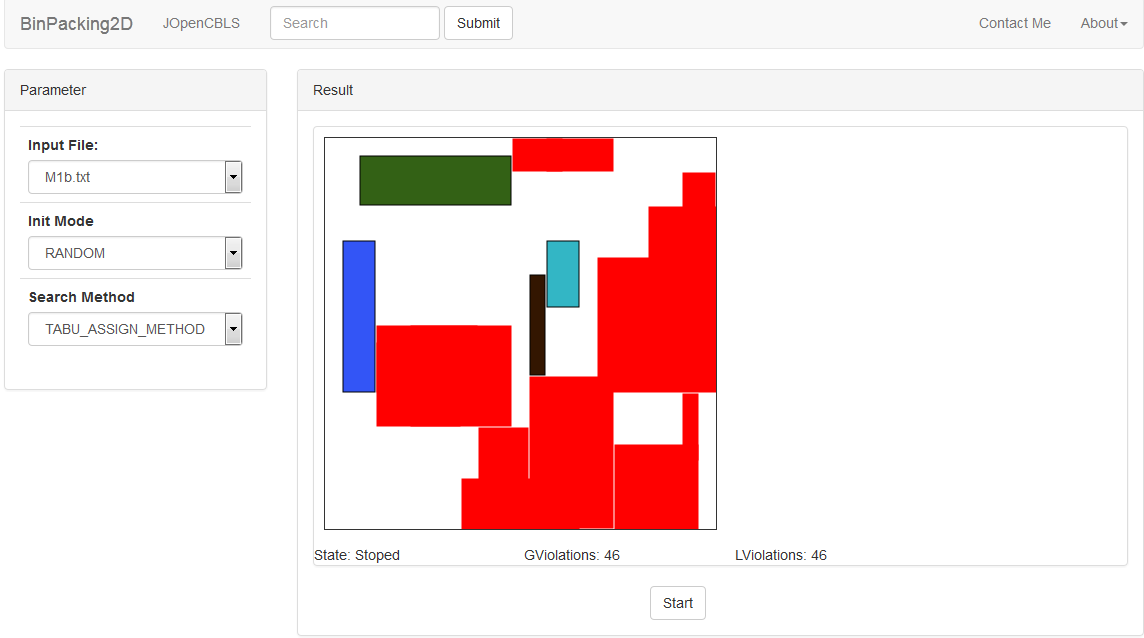
\includegraphics[scale=0.5]{figures/if-init.png}
	\caption{Giao diện khởi tạo chương trình \label{fig:ifInit}}
\end{figure}

Khi ứng dụng được khởi chạy, khi người dùng lựa chọn thay đổi bộ dữ liệu hoặc khi thay đổi thủ tục khởi tạo thì chương trình sẽ thực hiện khởi tạo mặc định các tham số và hiển thị lên màn hình như hình \ref{fig:ifInit}. Chương trình sẽ hiển thị các vật phẩm được xếp vào thùng không thỏa mãn các ràng buộc bởi màu đỏ, các vật thỏa mãn các ràng buộc sẽ được hiển thị bởi một màu nhẹ ngẫu nhiên.
\subsection*{Thực hiện tìm kiếm}
\begin{figure}
	\centering
	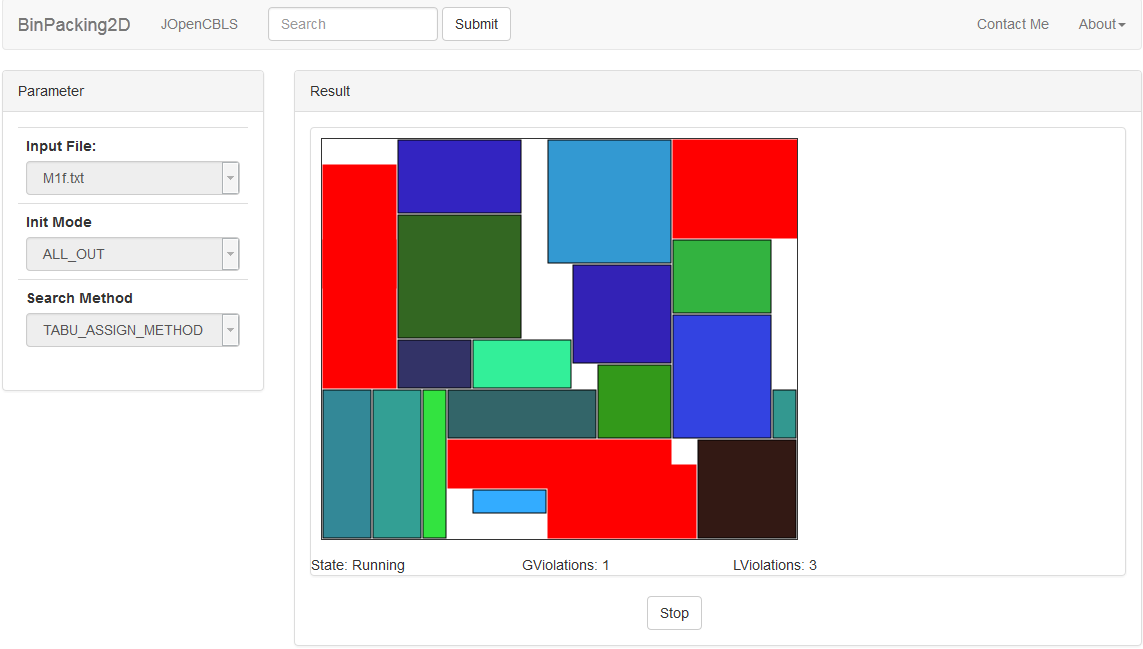
\includegraphics[scale=0.5]{figures/if-progress.png}
	\caption{Giao diện thực hiện tìm kiếm \label{fig:ifProgress}}
\end{figure}

Trong khi thực hiện tiến trình tìm kiếm, màn hình sẽ có dạng như hình \ref{fig:ifProgress}, nó sẽ thống kê số vi phạm hiện tại và số vi phạm tốt nhất tìm thấy trên hệ thống. Giao diện sẽ thay đổi theo trạng thái tìm kiếm hiện tại trên máy chủ.

\subsection*{Hiển thị kết quả}
\begin{figure}
	\centering
	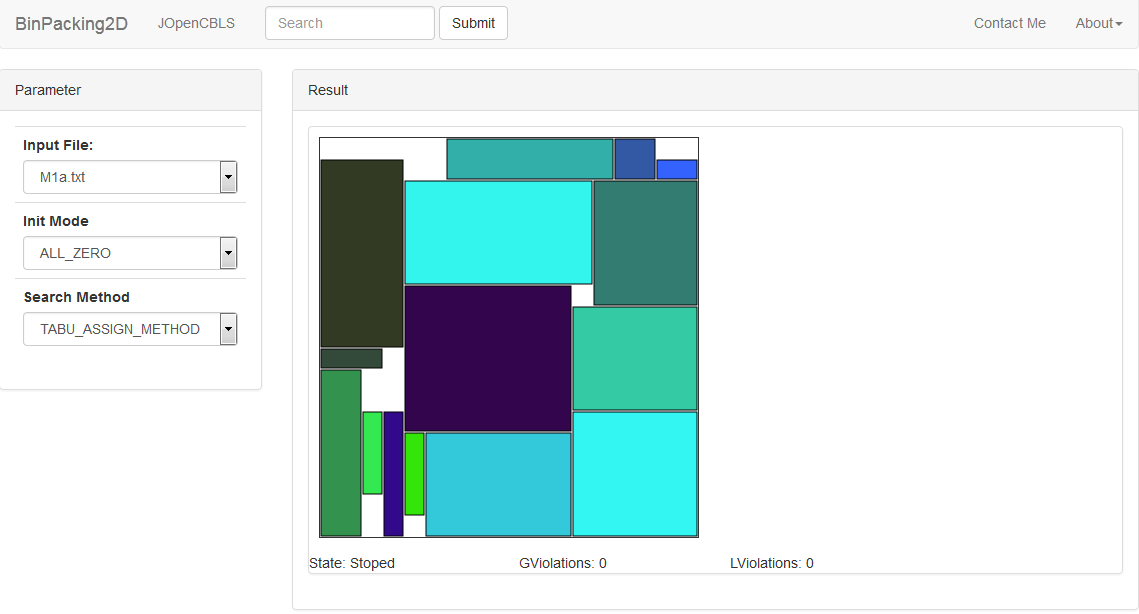
\includegraphics[scale=0.5]{figures/if-result.png}
	\caption{Giao diện kết quả chương trình \label{fig:ifResult}}
\end{figure}
Hình \ref{fig:ifResult} là giao diện sau khi thực hiện chương trình.
%==================================================================
\section{Kết quả thực nghiệm}
\subsection{Thực nghiệm}
Kết quả thực tế chạy trên các bộ dữ liệu mẫu được thống kê trong bảng \ref{tab:res}
{\scriptsize
\begin{table}[H]
	\centering
	\begin{threeparttable}
		%Thong ke thuat toan search asign
		\begin{tabular}{| l | c | c | c | c |}
			\hline
			\hline
			\multirow{ 2}{*}{Bộ DL\tnote{1}}
										& \multicolumn{2}{c}{RANDOM\tnote{2}} & \multicolumn{2}{c}{ALLZERO\tnote{2}} \\
			\cline{2-5}
										&Violations 		& Time(m)				& Violations		& Time (m)	\\
			\hline
			\hline

			M0a.txt 				 	&	0				&	1					& 	0			&	<1\\
			\hline
			M0b.txt 				 	&	0				&	10					& 	0			&	7\\
			\hline
			M1a.txt 				 	&	0				&	133					& 	0			&	19\\ 
			\hline
			M1b.txt 				 	&	0				&	243					& 	0			&	89\\ 
			\hline
			M1c.txt 					&	0				&	102					& 	0			&	267\\  
			\hline
			M1d.txt 					&	0				&	156					& 	0			&	78\\  
			\hline
			M1e.txt 					&	0\tnote{3}		&	378	    			& 	0\tnote{3}	&	326\\  
			\hline
			M1f.txt 					&	1				&	?					& 	1			&	?\\  
			\hline
			\hline
		\end{tabular}
		\begin{tablenotes}
			\item[1] Các bộ dữ liệu được cho trong \ref{tab:bpData}
			\item[2] Các số liệu được lấy từ giá trị trung bình 10 lần chạy trên mõi bộ dữ liệu bao gồm số bước lặp và thời gian thực thi.
			\item[3] Mục này chứa một vài lần thực thi cho kết quả vi phạm khác 0.
			\item[*] Kết quả thống kê được thực hiện trên máy tính intel với tốc độ xử lý 3.1GH với nền tảng Java 8.
		\end{tablenotes}
	\end{threeparttable}
    \caption{Kết quả thực thi trên các bộ dữ liệu mẫu của chương trình với thuật toán tìm kiếm Tabu cài đặt trong lớp \textsl{SearchTabuAssign} \label{tab:res}}

\end{table}
}

Các kết quả thống kê cho thấy bên cạnh thuật toán sẵn có trong thư viện JOpenCBLS thì các thuật toán cài đặt thêm đã cải thiện khá tốt khả năng tìm kiếm trong bài toán BP2D.

\subsection{Đánh giá chương trình}
\begin{itemize}
	\item \textbf{Ưu điểm}\\
	\begin{itemize}
		\item Giải quyết bài toán đóng thùng 2 chiều một cách có hiệu quả.
		\item Giao diện phầm mềm trực quan, dễ thao tác.
		\item Áp dụng nhiều công nghệ mới như AngularJS, Bootstrap, Java servlet, kiến trúc MVP để xây dựng chương trình.
		\item Sử dụng được tính mềm dẻo, tái sử dụng của thư viện JOpenCBLS.
	\end{itemize}
	\item \textbf{Nhược điểm}
	\begin{itemize}
		\item Chưa thực hiện và giải quyết trên bộ dữ liệu lớn.
	\end{itemize}
\end{itemize}
    %\chapter{Kết quả và hướng phát triển}
\label{chap:conc}

%=======================================================================
\section{Kết quả}

%=======================================================================
\section{Hướng phát triển}

Đồ án đã nghiên cứu thành công phương pháp giải bài toán đóng thùng với phương pháp tìm kiếm cục bộ dựa trên ràng buộc sử dụng thư viện JOpenCBLS của TS. Phạm Quang Dũng. Nhưng trong phạm vi đồ án tôi không phân tích sử dụng được hết mọi kỹ năng của thuật toán tìm kiếm cục bộ dựa trên ràng buộc cũng như không thể nghiên cứu rộng hơn về lớp các bài toán đóng thùng. Sau đây là những hướng mở rộng nghiên cứu của đồ án này:
\begin{itemize}
	\item Nghiên cứu thêm các Heuristic tìm kiếm mới hiệu quả hơn, góp phần cải thiện hiệu năng tìm kiếm trong các bài toán tìm kiếm cục bộ dựa trên ràng buộc.
	\item Phát triển đầy đủ bộ công cụ mô hình cho thư viện JOpenCBLS.
	\item Cải thiện hiệu quả của thuật toán đã cài đặt để có thể sử dụng tốt hơn cho các bộ dữ liệu lớn hơn.
	\item Mở rộng bài toán đóng thùng 2 chiều sang bài toán $n$ chiều và thỏa mãn thêm nhiều ràng buộc hơn:
	\begin{itemize}
		\item Ràng buộc thứ tự đặt các vật vào thùng.
		\item Ràng buộc yêu cầu xếp cạnh nhau các vật.
	\end{itemize}
	\item Phát triển bài toán đóng thùng với yêu cầu mới: lựa chọn số lượng các vật cho vào thùng để tối ưu một hay nhiều mục tiêu nào đó.
\end{itemize}
Tiếp tục nghiên cứu các kỹ thuật nhằm tăng hiệu quả của thuật toán, giải quyết tốt hơn các bộ dữ liệu lớn.





    \chapter*{Kết luận và hướng phát triển\markboth{Kết luận và hướng phát triển}{}}
\addcontentsline{toc}{chapter}{Kết luận và hướng phát triển}

%=======================================================================
\section*{Kết luận}

Đồ án tốt nghiệp với đề tài \textsc{Nghiên cứu và áp dụng thuật toán tìm kiếm cục bộ dựa trên ràng buộc để giải bài toán đóng thùng} đã hoàn thành các mục tiêu yêu cầu:
\begin{itemize}
	\item Nghiên cứu thuật toán tìm kiếm cục bộ để giải các bài toán thỏa mãn ràng buộc.
	\item Tìm hiểu và sử dụng thành thạo các thành phần của thư viện JOpenCBLS.
	\item Mô hình hóa và giải bài toán đóng thùng ở mức 2 chiều.
	\item Xây dựng ứng dụng Web sử dụng công nghệ JAVA và các công nghệ phía browser khác.
	\item Cài đặt các thuật toán tìm kiếm khác ngoài các thuật toán cài đặt sẵn để chạy thử, so sánh hiệu năng.
	\item Mở rộng thư viện JOpenCBLS để sử dụng tốt hơn trong các ứng dụng Web.
\end{itemize}
%=======================================================================

%=======================================================================
\section*{Hướng phát triển}

Đồ án đã nghiên cứu thành công phương pháp giải bài toán đóng thùng với phương pháp tìm kiếm cục bộ dựa trên ràng buộc sử dụng thư viện JOpenCBLS của TS. Phạm Quang Dũng. Nhưng trong phạm vi đồ án tôi không phân tích sử dụng được hết mọi kỹ năng của thuật toán tìm kiếm cục bộ dựa trên ràng buộc cũng như không thể nghiên cứu rộng hơn về lớp các bài toán đóng thùng. Sau đây là những hướng mở rộng nghiên cứu của đồ án này:
\begin{itemize}
	\item Nghiên cứu thêm các Heuristic tìm kiếm mới hiệu quả hơn, góp phần cải thiện hiệu năng tìm kiếm trong các bài toán tìm kiếm cục bộ dựa trên ràng buộc.
	\item Phát triển đầy đủ bộ công cụ mô hình cho thư viện JOpenCBLS.
	\item Cải thiện hiệu quả của thuật toán đã cài đặt để có thể sử dụng tốt hơn cho các bộ dữ liệu lớn hơn.
	\item Mở rộng bài toán đóng thùng 2 chiều sang bài toán $n$ chiều và thỏa mãn thêm nhiều ràng buộc hơn:
	\begin{itemize}
		\item Ràng buộc thứ tự đặt các vật vào thùng.
		\item Ràng buộc yêu cầu xếp cạnh nhau các vật.
	\end{itemize}
	\item Phát triển bài toán đóng thùng với yêu cầu mới: lựa chọn số lượng các vật cho vào thùng để tối ưu một hay nhiều mục tiêu nào đó.
\end{itemize}
Tiếp tục nghiên cứu các kỹ thuật nhằm tăng hiệu quả của thuật toán, giải quyết tốt hơn các bộ dữ liệu lớn.


    %\appendix
    \begin{appendices}
        \chapter{Dữ liệu kiểm tra}
\label{chap:cc}

{\scriptsize
\begin{table}[H]
    \centering
\begin{threeparttable}
   \begin{tabular}{| l | c | c | c | c ||}
			\hline
			\hline
			Bộ Dữ liệu					&	Chiều rộng BIN	& Chiều cao BIN		& Số vật phẩm\\
			\hline
			\hline
			M0a.txt 				 	&	9				&	7				& 	6\\ 
			\hline
			M0b.txt 				 	&	16				&	10				& 	10\\ 
			\hline
			M1a.txt 					&	18				&	19				& 	15\\  
			\hline
			M1b.txt 					&	23				&	23				& 	18\\  
			\hline
			M1c.txt 					&	23				&	24				& 	18\\  
			\hline
			M1d.txt 					&	24				&	25				& 	19\\  
			\hline
			M1e.txt 					&	20				&	21				& 	19\\  
			\hline
			M1f.txt 					&  	19				&	16				& 	21\\  
			\hline
		\end{tabular}
    	\caption{Kích thước và số lượng vật phẩm các bộ dữ liệu\label{tab:bpData}}
    
\end{threeparttable}
\end{table}
}% scriptsize

Bảng \ref{tab:bpData} liệt kê các thông tin đầu vào của các bộ dữ liệu sử dụng để đánh giá chương trình ứng dụng.

        %\include{chapters/Appendix2}
        %\include{chapters/Appendix3}
    \end{appendices}

%======================REFERENCE================================
\bibliographystyle{plain}
\bibliography{reference}

%==================================finish=========================

\end{document}
